%\documentclass[pdflatex,en,11pt]{aghdpl}
\documentclass[en]{aghdpl}
\usepackage[english]{babel}
\usepackage{polski}
\usepackage[utf8]{inputenc}

\usepackage[backend=biber,
style=numeric,
%bibencoding=ascii,
%style=reading
giveninits=true
]{biblatex}
\renewbibmacro{in:}{%
    \ifentrytype{article}{}{\printtext{\bibstring{in}\intitlepunct}}}

\addbibresource{bibliografia.bib}

\DeclareNameAlias{sortname}{last-first}
\DeclareNameAlias{default}{last-first}

% dodatkowe pakiety
\usepackage{enumerate}
\usepackage{listings}
\usepackage{float}
\usepackage[binary-units=true]{siunitx}
\usepackage{hyperref}
\usepackage[acronym,nomain,toc]{glossaries}
\usepackage{multirow}
\usepackage{colortbl}
\usepackage{hhline}
\usepackage{lscape}
\usepackage{csquotes}

% \lstloadlanguages{TeX}

\lstset{
  literate={ą}{{\k{a}}}1
           {ć}{{\'c}}1
           {ę}{{\k{e}}}1
           {ó}{{\'o}}1
           {ń}{{\'n}}1
           {ł}{{\l{}}}1
           {ś}{{\'s}}1
           {ź}{{\'z}}1
           {ż}{{\.z}}1
           {Ą}{{\k{A}}}1
           {Ć}{{\'C}}1
           {Ę}{{\k{E}}}1
           {Ó}{{\'O}}1
           {Ń}{{\'N}}1
           {Ł}{{\L{}}}1
           {Ś}{{\'S}}1
           {Ź}{{\'Z}}1
           {Ż}{{\.Z}}1
}

\newcommand{\rad}{\radian}
\newcommand{\iic}{$I^2C$}
\newcommand{\uA}{\micro\ampere}
\newcommand{\mA}{\milli\ampere}
\newcommand{\uV}{\micro\volt}
\newcommand{\mV}{\milli\volt}
\newcommand{\Hz}{\hertz}
\newcommand{\kHz}{\kilo\hertz}
\newcommand{\MHz}{\mega\hertz}
\newcommand{\bps}{\bit / \second}
\newcommand{\Bps}{\byte / \second}
\newcommand{\kbps}{\kilo\bps}
\newcommand{\kBps}{\kilo\Bps}
\newcommand{\Mbps}{\mega\bps}
\DeclareSIUnit{\belmilliwatt}{Bm}
\DeclareSIUnit{\belisotropic}{Bi}
\DeclareSIUnit{\dBm}{\deci\belmilliwatt}
\DeclareSIUnit{\dBi}{\deci\belisotropic}
\DeclareSIUnit{\ppm}{ppm}

\usepackage{array}
\newcolumntype{L}[1]{>{\raggedright\let\newline\\\arraybackslash\hspace{0pt}}m{#1}}
\newcolumntype{C}[1]{>{\centering\let\newline\\\arraybackslash\hspace{0pt}}m{#1}}
\newcolumntype{R}[1]{>{\raggedleft\let\newline\\\arraybackslash\hspace{0pt}}m{#1}}

\makeatletter
\let\ps@plain\ps@fancy
\makeatother

%---------------------------------------------------------------------------

\author{Grzegorz Gajoch}
\shortauthor{G. Gajoch}

\course{Elektronika i Telekomunikacja}

\titlePL{System komunikacji satelity PW-Sat2}
\titleEN{PW-Sat2 satellite communication system}

\shorttitlePL{System komunikacji satelity PW-Sat2} % skrócona wersja tytułu jeśli jest bardzo długi
\shorttitleEN{PW-Sat2 satellite communication system}

\thesistypePL{Praca dyplomowa magisterska}
\thesistypeEN{Master Thesis}

\supervisorPL{dr inż. Cezary Worek}
\supervisorEN{Cezary Worek Ph.D}

\date{2019}

\departmentPL{Katedra Elektroniki}
\departmentEN{Department of Electronics}

\facultyPL{Wydział Informatyki, Elektroniki i Telekomunikacji}
\facultyEN{Faculty of Computer Science, Electronics and Telecommunications}

\acknowledgements{}

\setlength{\cftsecnumwidth}{10mm}


\makeatletter
\newcommand*{\marker}[1][]{%
  \begingroup
    \edef\x{\the\pdfelapsedtime}%
    \count@\x\relax
    \divide\count@\p@
    \edef\s{\the\count@}%
    \count@\s\relax
    \divide\count@ 60 %
    \edef\m{\the\count@}%
    \count@\m\relax
    \divide\count@ 60 %
    \edef\h{\the\count@}%
    \edef\s{\the\numexpr\x-65536*60*\m}%
    \dimen@\s sp %
    \edef\s{\ifdim\dimen@<10pt 0\fi\strip@pt\dimen@}%
    \edef\m{\the\numexpr\m-60*\h}%
    \edef\m{\ifnum\m<10 0\fi\m}%
    \edef\timestamp{\h:\m:\s}%
    \immediate\write16{%
      [\timestamp] #1%
    }%
  \endgroup
}
\makeatother

%---------------------------------------------------------------------------

\begin{document}

\marker[timetimetime-00-begin]

\titlepages
\tableofcontents
\clearpage

\marker[timetimetime-0-before]

\chapter{Introduction}

In satellite applications, radio communication is the most important method for controlling the satellite state and issuing any commands to it. 

\section{Aim of the thesis}

The aim of this thesis was to design, test \& deploy communication system for second Polish satellite, PW-Sat2. This work covers phases of component selection \& design, testing all the subsystems and finally results from the on-orbit mission.

\section{PW-Sat2}
    The presented system was design specifically to be deployed on-board the PW-Sat2 satellite \cite{PW-Sat2URL}. PW-Sat2 was launched on Low Earth Orbit or 3rd of December 2018 on-board Falon9 rocket from SpaceX company.

    In the figure \ref{PW-Sat_render_01} an exploded render of PW-Sat2 is presented.
    
    %%% [TODO]: JAKIEŚ ZDJĘCIA

    \begin{figure}[H]
        \centering
        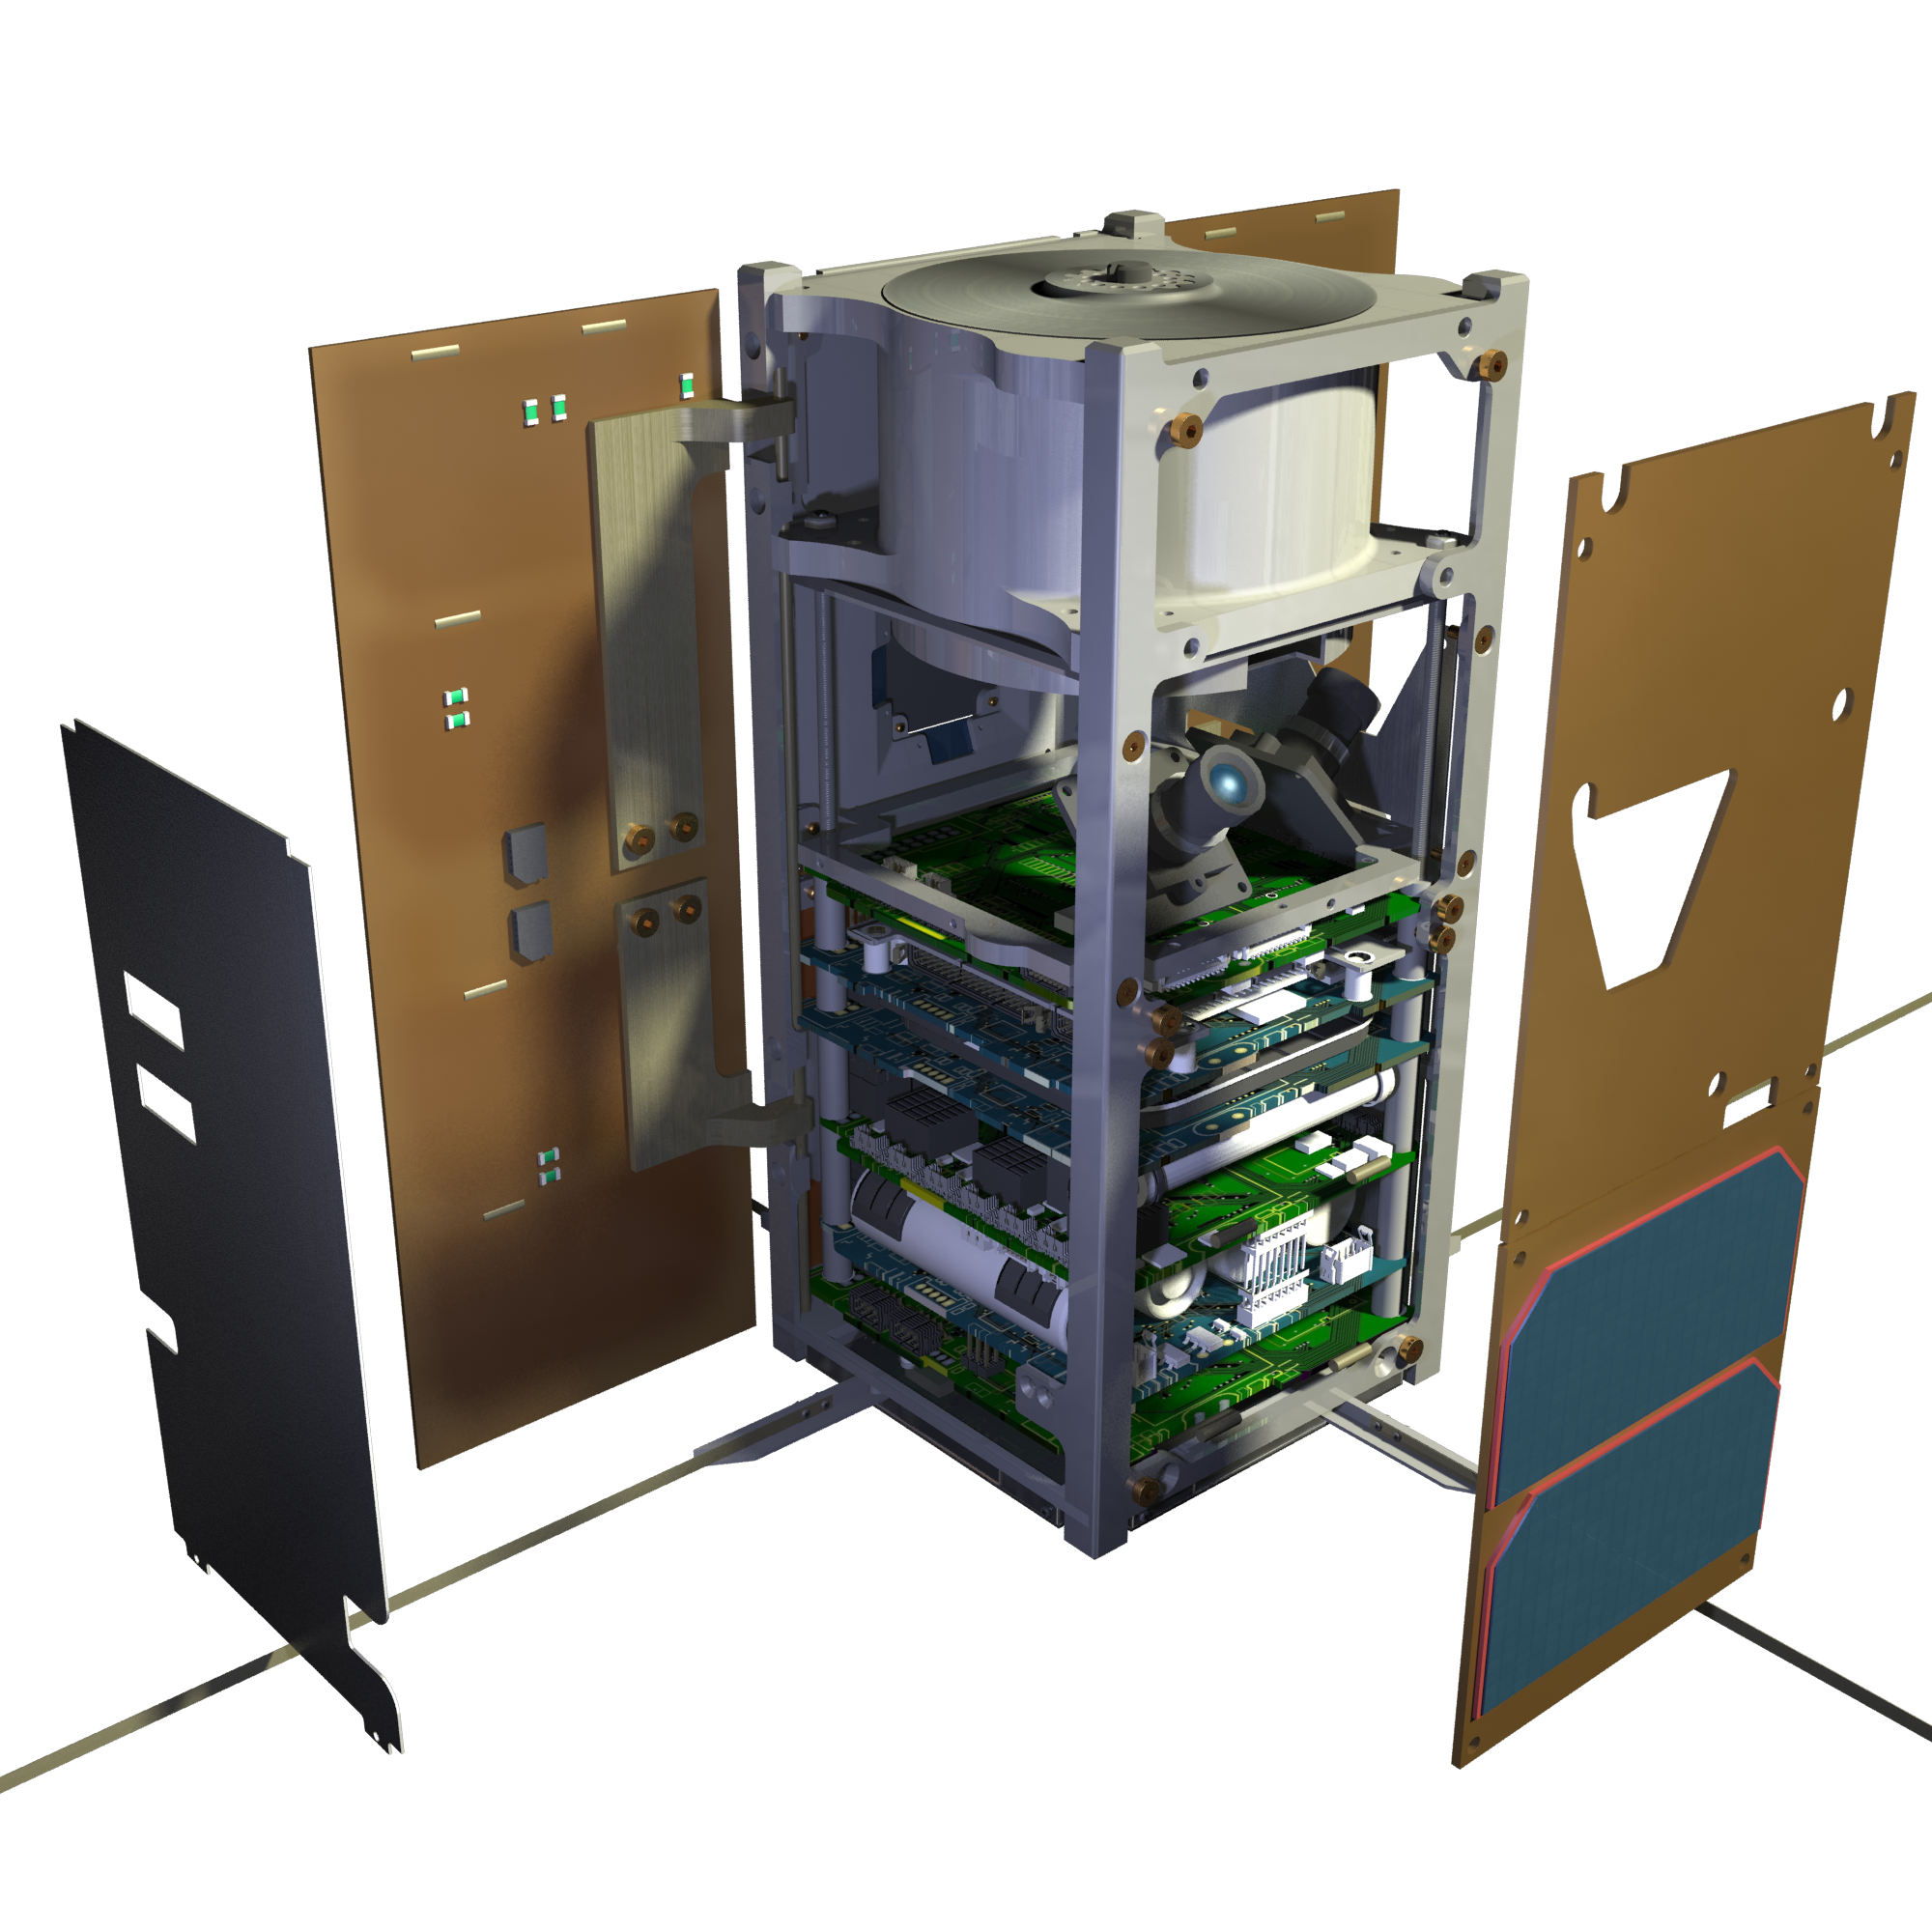
\includegraphics[width=0.65\paperwidth]{img/4/PW-Sat2_render_01.png}
        \caption{PW-Sat2 render. Source: \cite{PW_sat2_photo}}
        \label{PW-Sat_render_01}
    \end{figure}


    \subsection{Primary mission}
    % skopiowane z inż, do przepisania
        The primary mission of PW-Sat2 is to test the deorbit sail. When satellite mission ends, it has to be safely deorbited (or moved to graveyard orbit). Due to new regulations, satellite has to be removed from
        the LEO region no later than 25 years after the end of vehicle operations \cite{Satellite_disposal}. Purpose of deorbit sail is, after satellite operations, to open and increase atmospheric drag, shortening satellite life and cause deorbitation. More information about this experiment can be found in \cite{DDC_article}.

        A render of PW-Sat2 with opened sail is shown in the figure \ref{PW-Sat_render_sail}.

        \begin{figure}[H]
            \centering
            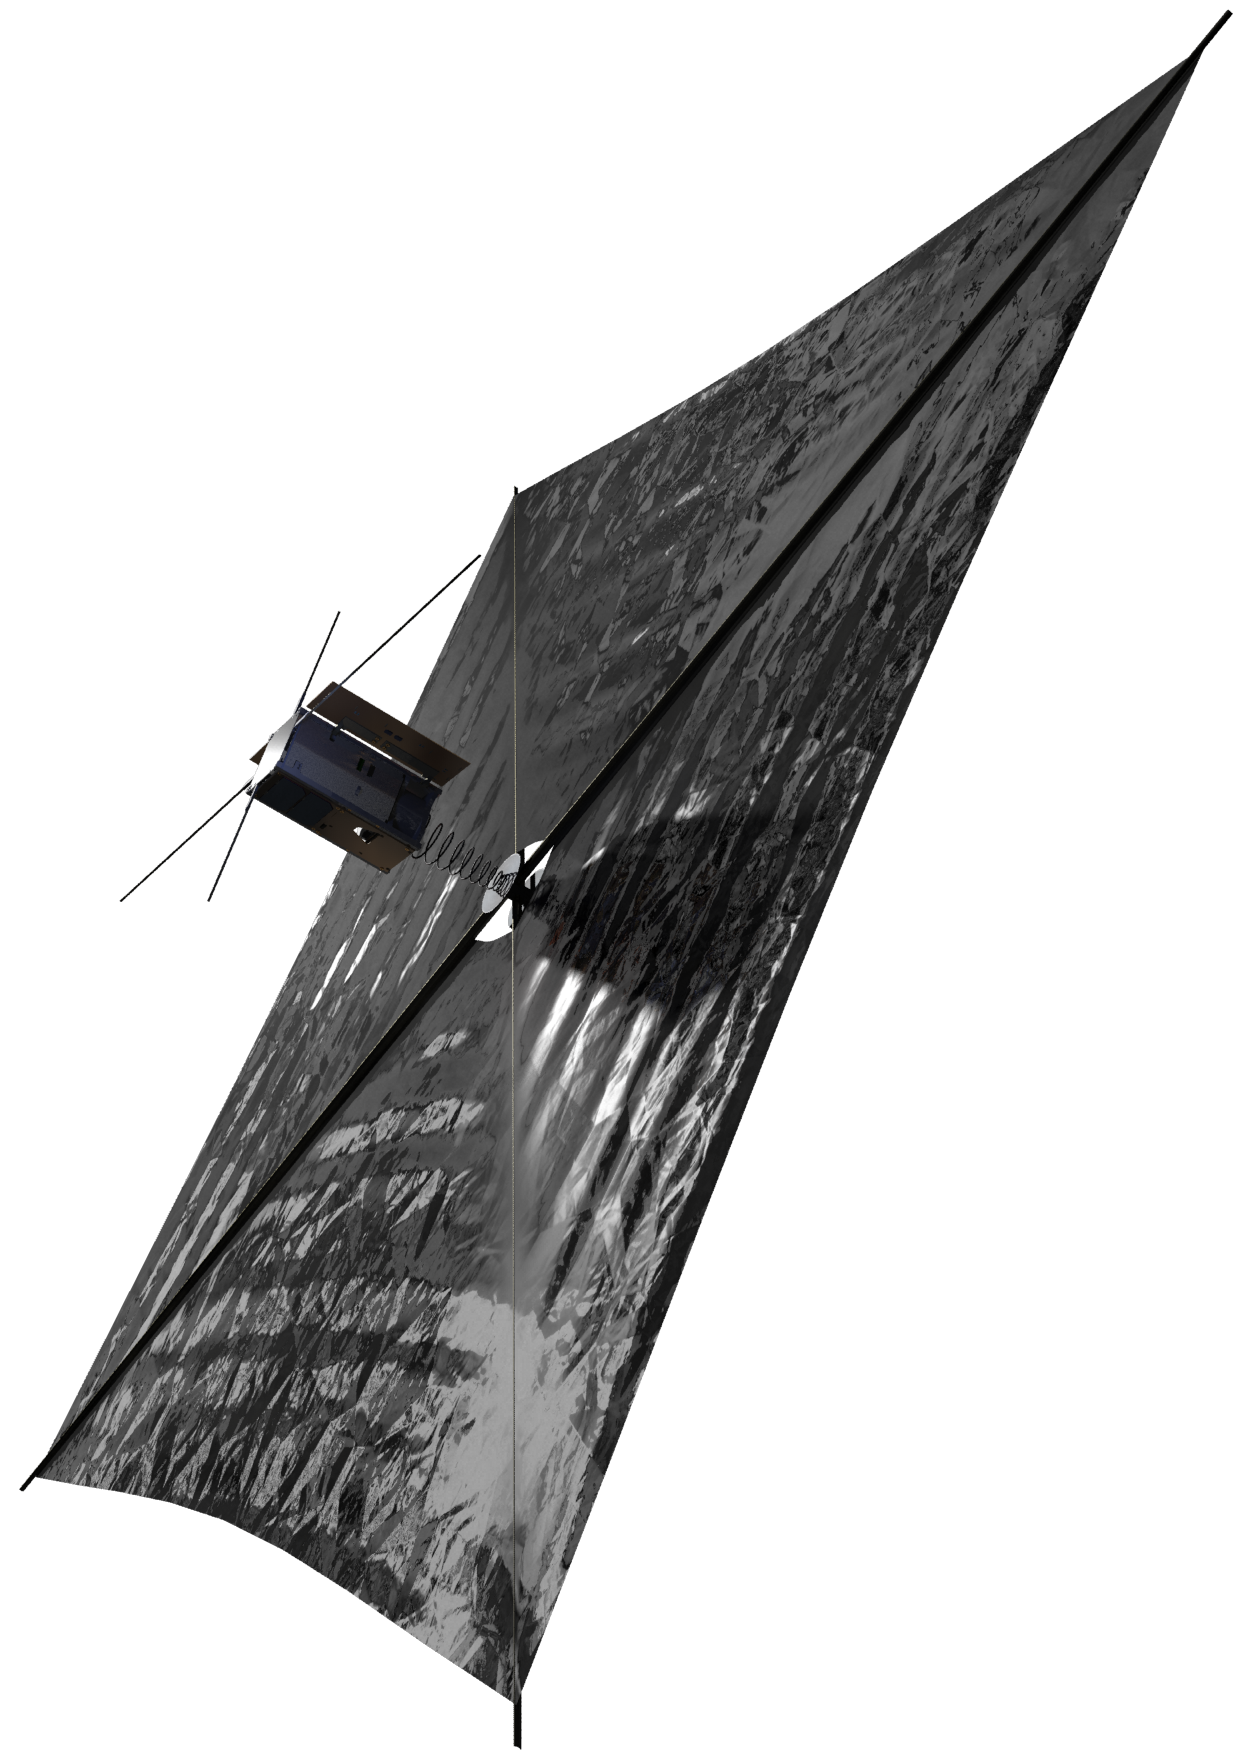
\includegraphics[width=0.38\paperwidth]{img/4/PW-Sat2_render_02.png}
            \caption{PW-Sat2 with opened sail. Source: \cite{PW_sat2_photo}}
            \label{PW-Sat_render_sail}
        \end{figure}

    \subsection{Mission plan and system lifetime}
        PW-Sat2 mission was divided into two phases: normal \& extended mission. Normal phase was planned to take 40 days, after which the deorbitation phase and extended mission begin. Deorbitation can  take up two two years, during which its state along with satellite housekeeping should be monitored.

    \subsection{Orbit}
        PW-Sat2 in planned to be launched to a sun-synchronous circular orbit of attitude \SI{575}{\kilo\meter}, with LTAN of 10:30 \cite{PWSAT_MA_CDR}.



\section{Low Earth Orbit satellite communication review}



\section{Requirements for the system}
\marker[timetimetime-1-introduction]

\chapter{Radio communication with the nanosatellites - state of the art}

\section{Subsystem review}
There are number of commercially available solutions and subsystems. Usually they are divided into subsystems, allowing user to mix different suppliers depending on the requirements, assuring they are compatible.

\subsection{Cubesat commmunication diagram}
Typical Low Earth Orbit satellite communication systems is shown in the figure \ref{comm_diagram}.

\begin{figure}[H]
    \centering
    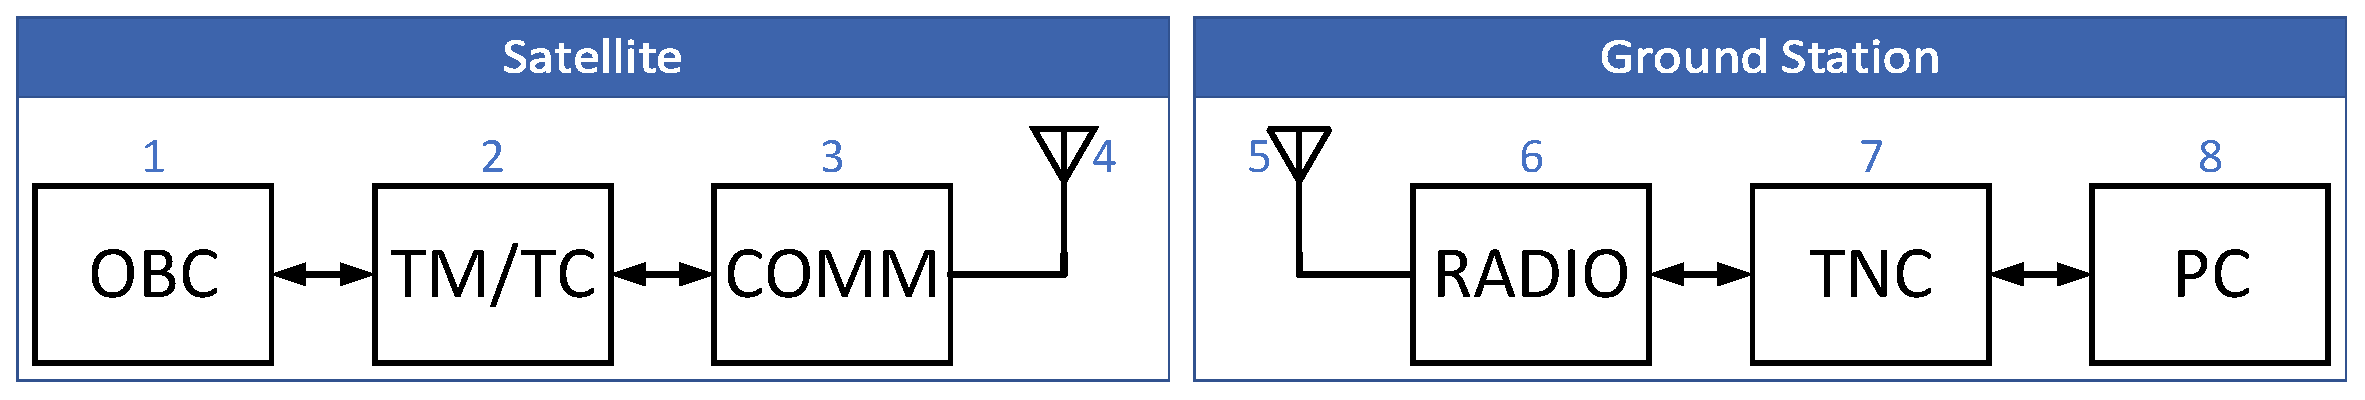
\includegraphics[width=0.7\paperwidth]{img/2/comm_diagram.eps}
    \caption{General communication system diagram}
    \label{comm_diagram}
\end{figure}

It consists of:
\begin{enumerate}
    \item On-Board Computer - controls the satellite, generates data and receives telecommands,
    \item Telemetry/Telecommand generator - translates between packets and baseband signal (modulator and demodulator),
    \item COMM - communications module, performs up/down conversion, amplification and antenna matching, usually on smaller missions it is integrated with TMTC on one module,
    \item Satellite antenna(s), typically omnidirectional to provide coverage during random satellite tumbling
    \item Ground station antenna(s), directional to maximize gain of the radio link,
    \item RADIO - radio system, typically a low noise amplifier with up/down converter and modulator, converts radio frequencies to baseband signals,
    \item Terimnal Network Controller - translates between packets and baseband signal, can be done as a separate device or in software in the PC,
    \item PC - a computer, which operator of the satellite uses to generate and receive data packets.
\end{enumerate}

\subsection{Cubesat antennas}
Cubesat dimensions are strict and defined in the CubeSat Design Specification \cite{cubesat_spec} as \si{100}x\si{100}~mm square \ref{CubeSat_max_dim}. This poses a requirement of antenna unfolding for antennas larger than side width. Usually this is required for all sub-GHz band, such as considered VHF and UHF bands. Higher bands, such an S-band, usually use patch antennas mounted on the wall.

\begin{figure}[H]
    \centering
    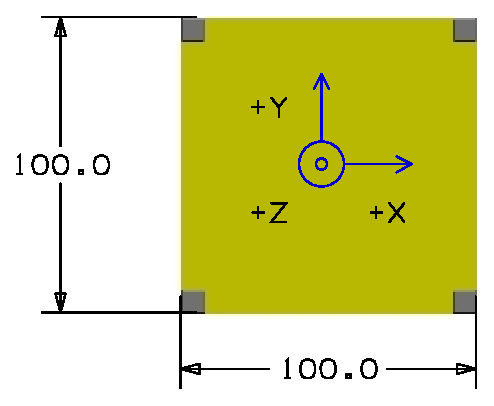
\includegraphics[width=0.5\paperwidth]{img/2/cubesat_dimensions.eps}
    \caption{CubeSat maximum dimensions, top view. Source \cite{cubesat_spec}.}.
    \label{CubeSat_max_dim}
\end{figure}

Antennas are usually unfolded by the spring action of the antennas itself and they are released by the on-board computer (by the thermal knife). Three typical antenna deployment systems are shown in the figures \ref{stiff_antenna_pic}, \ref{m_cubed}, \ref{isis_dipole_antenna}.

Typical unidirectional VHF/UHF antennas are dipoles, monopoles or turnstille. Selecting one depends on the mission requirements and link budget. Turnstille antenna, providing best link budget and circular polarization require that radiation elements are mounted on two sides of the CubeSat. Dipole option uses two elements is not as dependent on the ground reference (main structure) as the monopole antenna.

\begin{figure}[H]
    \centering
    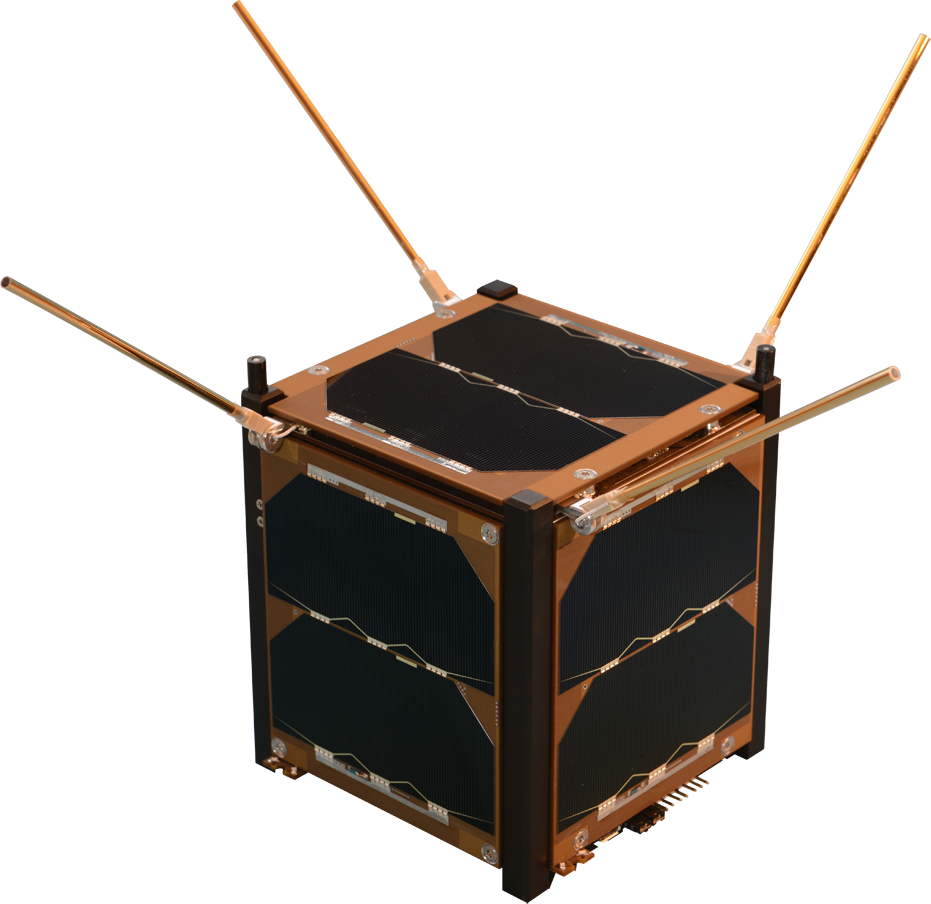
\includegraphics[width=0.5\paperwidth]{img/2/antenna_stiff.png}
    \caption{Deployed stiff antenna. In the stowed configuration they are along the solar panels. Source \cite{stiff_antenna_paper}.}.
    \label{stiff_antenna_pic}
\end{figure}

\begin{figure}[H]
    \centering
    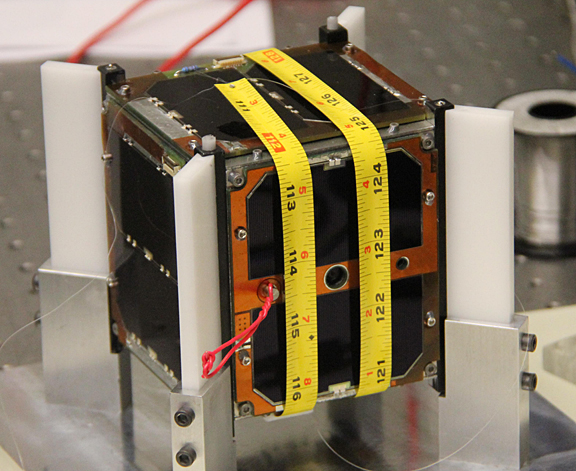
\includegraphics[width=0.5\paperwidth]{img/2/m-cubed.jpg}
    \caption{Tape measure antenna in the stowed configuration. Flat spring action forces antenna to deploy itself after its release. Source \cite{m_cubed}.}.
    \label{m_cubed}
\end{figure}

\begin{figure}[H]
    \centering
    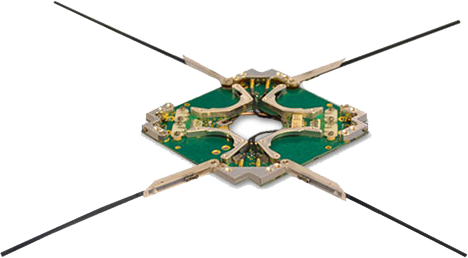
\includegraphics[width=0.5\paperwidth]{img/2/isis_dipole.png}
    \caption{Flat spring antennas rolled inside the CubeSat square. Released by the thermal knife burning the lock of the antenna doors. Source \cite{isis_dipole_antenna}.}.
    \label{isis_dipole_antenna}
\end{figure}

\subsection{Ground station antennas}
Space communication antennas require very large gain due to the distance between the stations and the omnidirectivity of the CubeSat antennas. Transmit power of the satellite is usually rather low (\SI{1}{\watt} or less).

Most of the designs use Yagi-Uda antennas, in circular polarization (cross-yagi with phasing). They are typically 9-11 elements long for VHF and 17-19 elements for UHF. Yagi-Uda antennas can be also phased as an array of antennas (1x2, 2x2 configuration etc.) improving gain and directivity. This however requires the antenna mast to withstand the size and weight of the system. Required power gain is dependent on the mission itself and the reliability of the link. Random tumbling and CubeSat antennas with dips in the radiation pattern (as monopole and dipole) require more directivity and power gain than attitude-controlled satellites. Direcitivity of the antenna also affects antenna noise temperature.

Depending on the mission, one, two or more antennas can be required due to the number of bands used. 

Due to the directivity of the antennas, their half-power beam width is around \si{2}-\SI{10}{\degree}. Therefore another required element of the ground station is the antenna rotator, which has to support the required weight, size and the location of the ground station.

In the figure \ref{isis_gs} the commercially available ISIS VHF/UHF ground station is shown, which employs two cross-yagi antennas (VHF, UHF), antenna mast and rotator and rotator controller.

\begin{figure}[H]
    \centering
    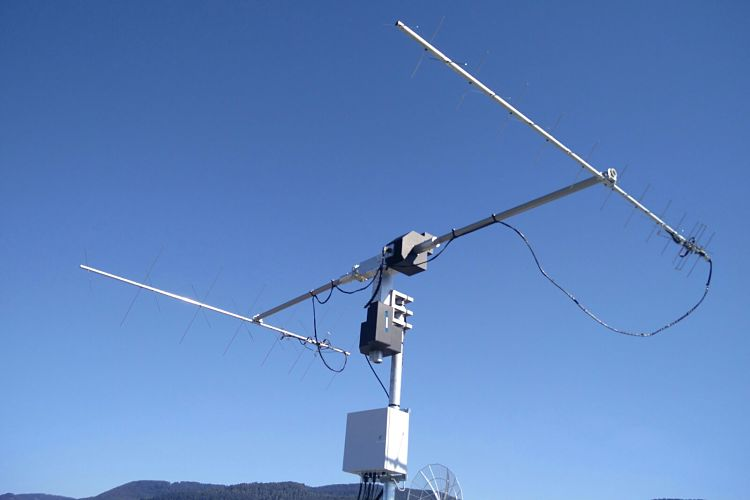
\includegraphics[width=0.5\paperwidth]{img/2/isis_gs.jpg}
    \caption{ISIS Ground Station. Source \cite{isis_gs}.}.
    \label{isis_gs}
\end{figure}

\subsection{Satellite communication subsystem}
Communication subsystem of the satellite is responsible of transmitting and receiving radio signals, modulating/demodulating them and providing data link for the On Board Computer. It has to be compatible with selected mechanical configuration, available data interfaces and the antennas to be installed. Most of the designs use custom design radio systems, using heterodyne receivers/transmitters (Fig. \ref{clyde_comm}), however there are an Software-Defined Radio systems, such as Gomspace SDR Platform \ref{gomspace_comm}.

\begin{minipage}{\linewidth}
    \centering
    \begin{minipage}{0.45\linewidth}
        \begin{figure}[H]
            \centering
            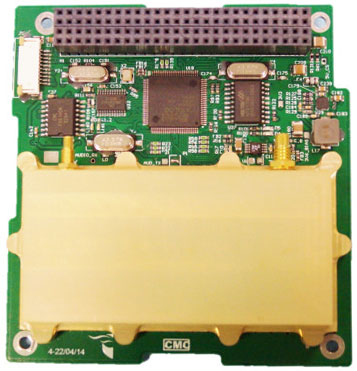
\includegraphics[width=0.32\paperwidth]{img/2/clyde_comm.jpg}
            \caption{CPUT UTRX from Clyde Space. Source: \cite{clyde_comm}}
            \label{clyde_comm}
        \end{figure}
    \end{minipage}
    \hspace{0.05\linewidth}
    \begin{minipage}{0.45\linewidth}
        \begin{figure}[H]
            \centering
            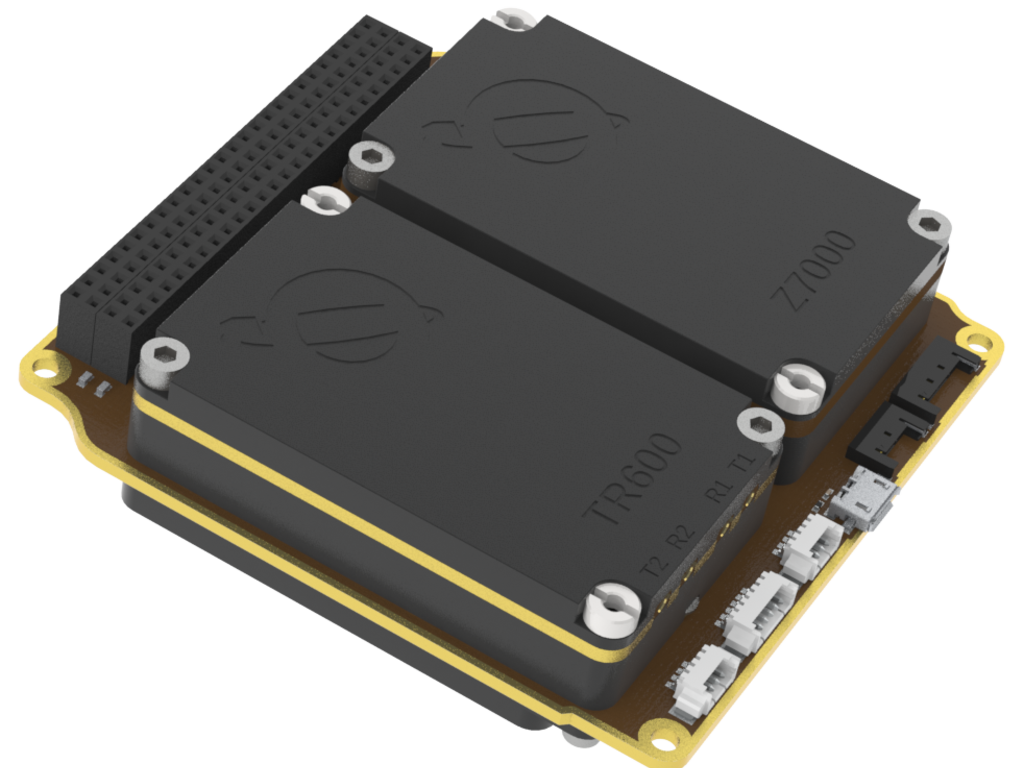
\includegraphics[width=0.35\paperwidth]{img/2/gomspace_sdr.png}
            \caption{Space qualified Software Defined Radio (SDR) Platform. Source: \cite{gomspace_comm}}
            \label{gomspace_comm}
        \end{figure}
    \end{minipage}
\end{minipage}


\subsection{Ground segment communication subsystem}
\subsubsection{Transmitter}
Due to the typically lower sensitivity and omnidirectional antenna on the satellite the uplink EIRP has to be very large, requiring not only directional antennas but also high output power (\si{100}-\SI{1500}{\watt}).
Depending on the modulation required, relatively cheap radio amateur transceivers can be used to modulate and amplify transmit signals, such as ICOM 910H or KENWOOD TS-2000 E (Fig. \ref{kenwood_ts2000}). As those types of radios were designed to transmit speech (bandwidth up to about \SI{10}{\kHz}) they can be used only to transmit signals which are FM, AM or SSB modulated. For other modulation and/or bandwidth the radio signal has to be generated by other type of radio (integrated or software-defined) and power amplifier.

Depending on the required output power, high-power amplifier can be used to further increase output power up to several kilo-watts. 

\begin{minipage}{\linewidth}
    \centering
    \begin{minipage}{0.45\linewidth}
        \begin{figure}[H]
            \centering
            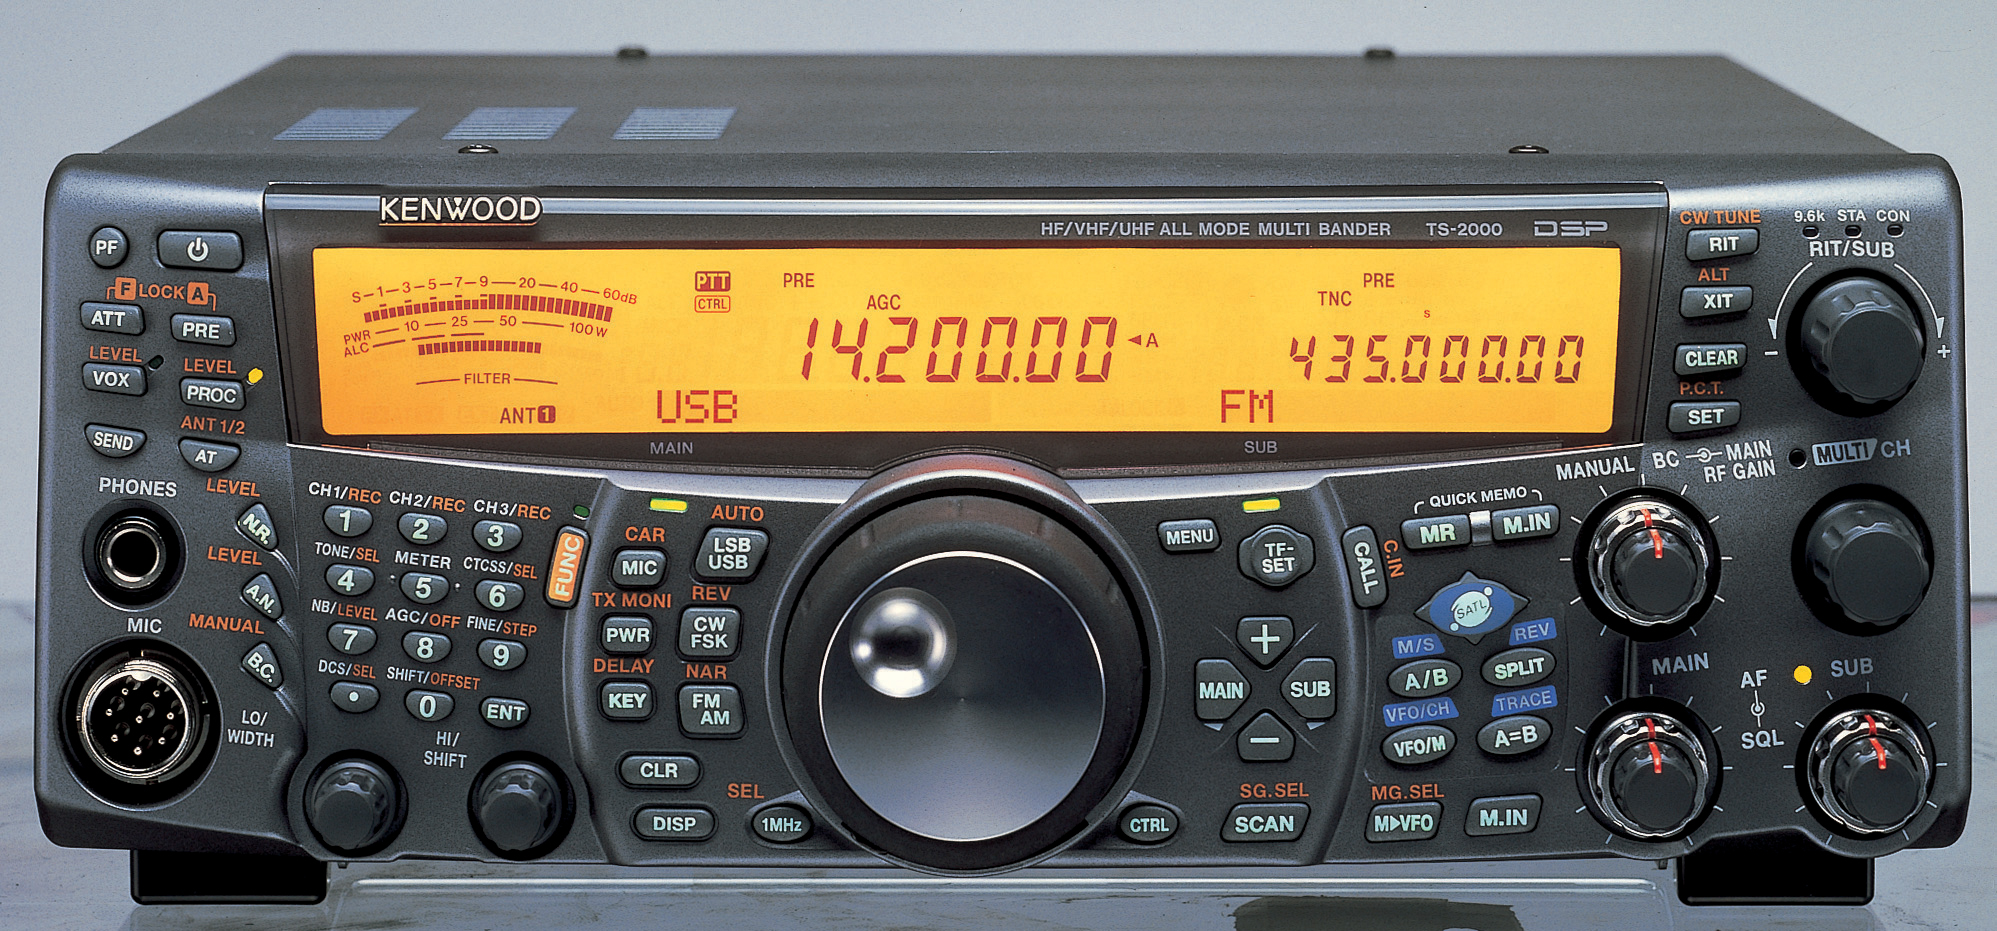
\includegraphics[width=0.35\paperwidth]{img/2/kenwood_ts2000.jpg}
            \caption{KENWOOD TS-2000 E all mode transceiver. Source: \cite{kenwood_ts2000}}
            \label{kenwood_ts2000}
        \end{figure}
    \end{minipage}
    \hspace{0.05\linewidth}
    \begin{minipage}{0.45\linewidth}
        \begin{figure}[H]
            \centering
            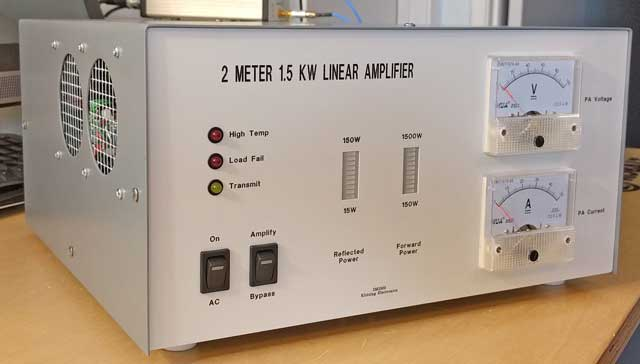
\includegraphics[width=0.35\paperwidth]{img/2/vhf_1500w_pa.jpg}
            \caption{\SI{1500}{\watt} VHF power amplifier. Source: \cite{vhf_1500w_pa}}
            \label{vhf_1500w_pa}
        \end{figure}
    \end{minipage}
\end{minipage}

\subsubsection{Receiver}
The receiver on the ground has to complement the space segment. Due to relatively low transmit power on the satellite, the receiver sensitivity should be very high. Additionally, receiver intermodulation performance should withstand possible blocking signals which are present on the ground.

To increase the sensitivity, Low Noise Amplifier has to be installed close to the antenna, such as LNA SSB-70 for UHF band (Fig. \ref{TODO}), which has Noise Figure of about \SI{0.35}{\dB}. Intermodulation and blocking is provided at the first stage by placing low-loss filter before the LNA, such as Cavity filters (Fig. \ref{cavity_uhf}).

\begin{minipage}{\linewidth}
    \centering
    \begin{minipage}{0.45\linewidth}
        \begin{figure}[H]
            \centering
            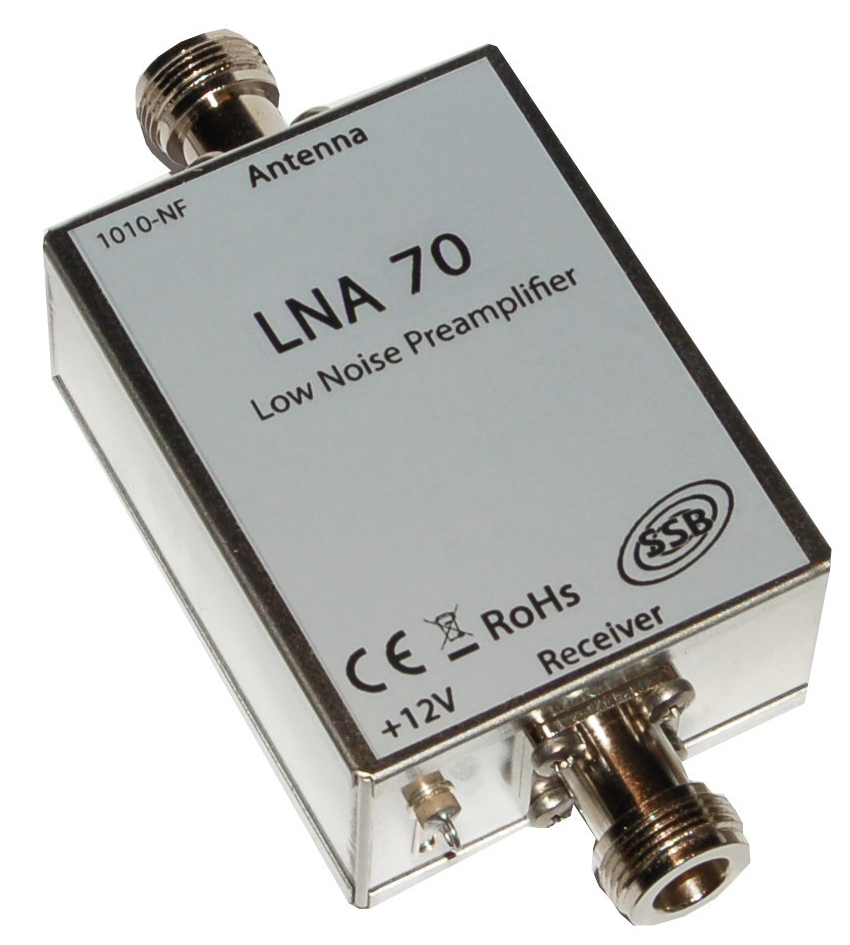
\includegraphics[width=0.3\paperwidth]{img/2/ssb_lna70.jpg}
            \caption{LNA SSB-70 Low Noise Amplifier for UHF band. Source: \cite{ssb_lna70}}
            \label{ssb_lna70}
        \end{figure}
    \end{minipage}
    \hspace{0.05\linewidth}
    \begin{minipage}{0.45\linewidth}
        \begin{figure}[H]
            \centering
            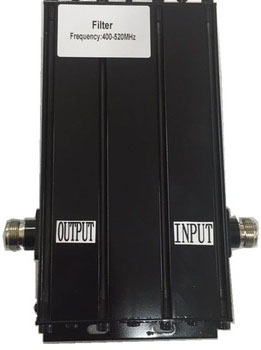
\includegraphics[width=0.1\paperwidth]{img/2/cavity_uhf.jpg}
            \caption{LBQ-450 3-cavity UHF bandpass filter. Source: \cite{cavity_uhf}}
            \label{cavity_uhf}
        \end{figure}
    \end{minipage}
\end{minipage}

Radio signal, pre-amplified by the low-noise amplifier is down-converted to the baseband and de-modulated. This can be performed by the integrated radio transceiver (same as the transmitter, this emposes the same modulation constraints as for the transmitter) or by the software-defined radio, such as an NI-USRP 2901 (Fig. \ref{ni_2901}) or FUNCube Dongle Pro+ (which was specifically designed for the FUNCube CubeSat - Fig. \ref{funcube}).

\begin{minipage}{\linewidth}
    \centering
    \begin{minipage}{0.45\linewidth}
        \begin{figure}[H]
            \centering
            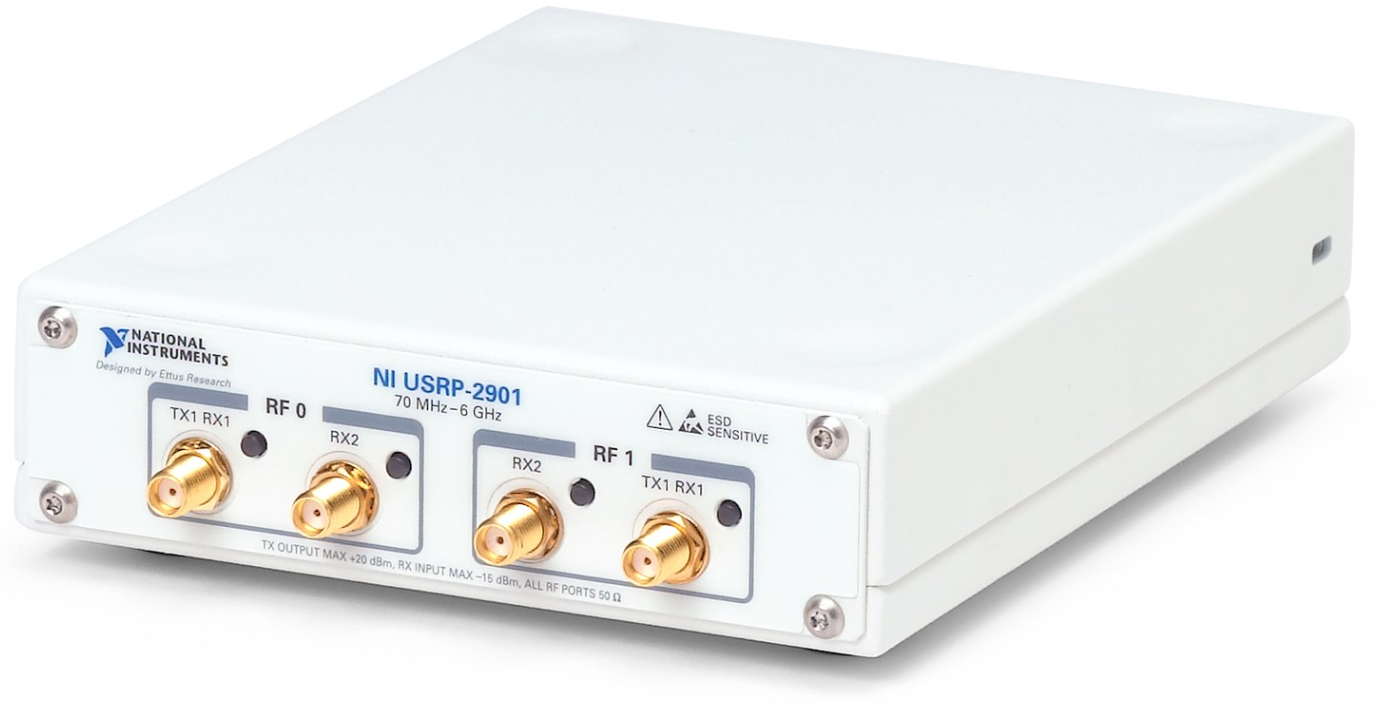
\includegraphics[width=0.3\paperwidth]{img/2/ni_2901.png}
            \caption{USRP-2901 Software Defined Radio Device. Source: \cite{ni_2901}}
            \label{ni_2901}
        \end{figure}
    \end{minipage}
    \hspace{0.05\linewidth}
    \begin{minipage}{0.45\linewidth}
        \begin{figure}[H]
            \centering
            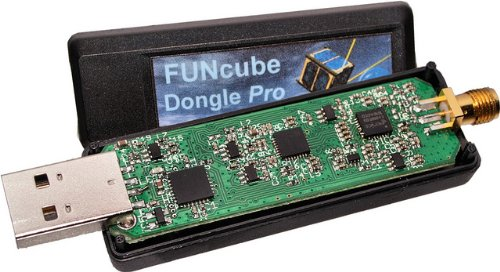
\includegraphics[width=0.3\paperwidth]{img/2/funcube.jpg}
            \caption{FUNcube Dongle Pro+. Source: \cite{funcube}}
            \label{funcube}
        \end{figure}
    \end{minipage}
\end{minipage}

After down-conversion baseband signal has to be de-modulated, which is done by the Terminal Network Controller. This can be implemeneted as a custom hardware solution (analog-to-digital converter and custom digital signal processor, for example TNC-X shown in the figure \ref{tncx}) or by pure software. Software solution has more flexibility but require a PC to perform signal processing, as is the only option for software-defined radio. One of the available TNC software using audio card is the Direwolf \cite{direwolf}.

\begin{figure}[H]
    \centering
    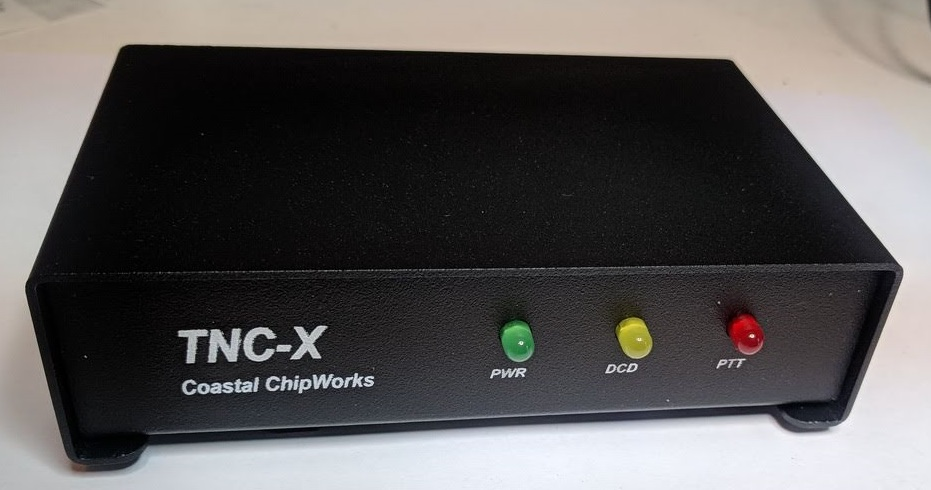
\includegraphics[width=0.3\paperwidth]{img/2/tncx.jpg}
    \caption{Terminal Network Controller TNC-X. Source: \cite{tncx}}
    \label{tncx}
\end{figure}



\section{Similar missions and designs}
In this section, three already flown satellite missions are described: PW-Sat, SwissCube and MOVE-I. 
\subsection{PW-Sat}
First polish satellite, PW-Sat, was launched in year \si{2012}. It was build on Warsaw Univeristy of Technology, with Space Research Centre PAS support. 

PW-Sat used ISIS TRXUV on-board communication module, with two (UHF uplink + VHF downlink) dipoles. Used modulations were AFSK \SI{1200}{\bps}. Radio transmit output power was \SI{30}{\dBm}. 
Ground station was built on Nicolaus Copernicus Astronomical Center in Warsaw, using \si{4}, \si{9}~element synphase cross-yagi VHF antennas for downlink and \si{4}, \si{19}~element synphase cross-yagi UHF antennas for uplink. Peak output power for uplink was \SI{100}{\watt} from the ICOM 910H transceiver.

PW-Sat and its ground station antennas are shown in the figures \ref{PW-Sat1_pic} and \ref{CAMK_pic}.

\begin{minipage}{\linewidth}
    \centering
    \begin{minipage}{0.45\linewidth}
        \begin{figure}[H]
            \centering
            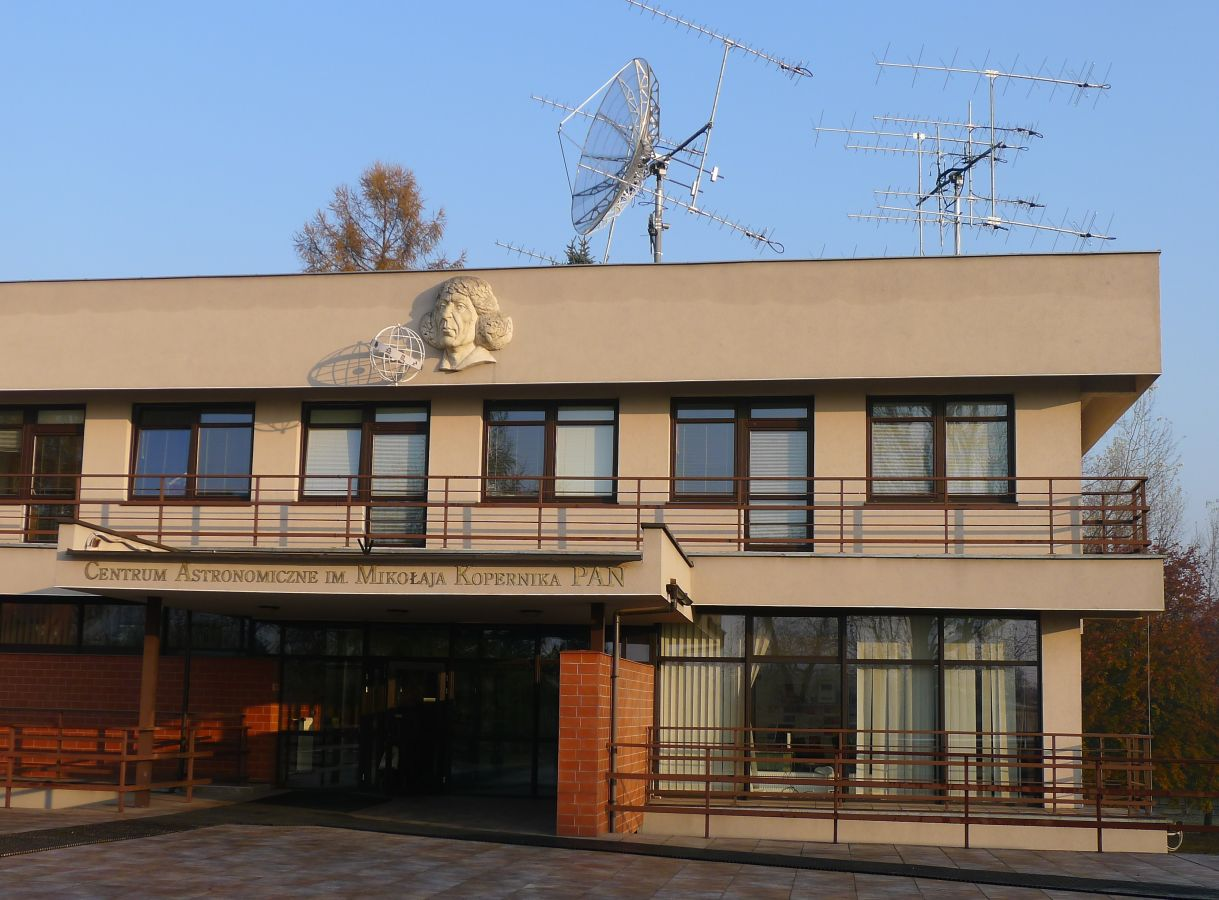
\includegraphics[width=0.32\paperwidth]{img/2/camk_pic.jpg}
            \caption{Nicolaus Copernicus Astronomical Center in Warsaw. PW-Sat antennas on the right. Source: \cite{camk_pic}}
            \label{CAMK_pic}
        \end{figure}
    \end{minipage}
    \hspace{0.05\linewidth}
    \begin{minipage}{0.45\linewidth}
        \begin{figure}[H]
            \centering
            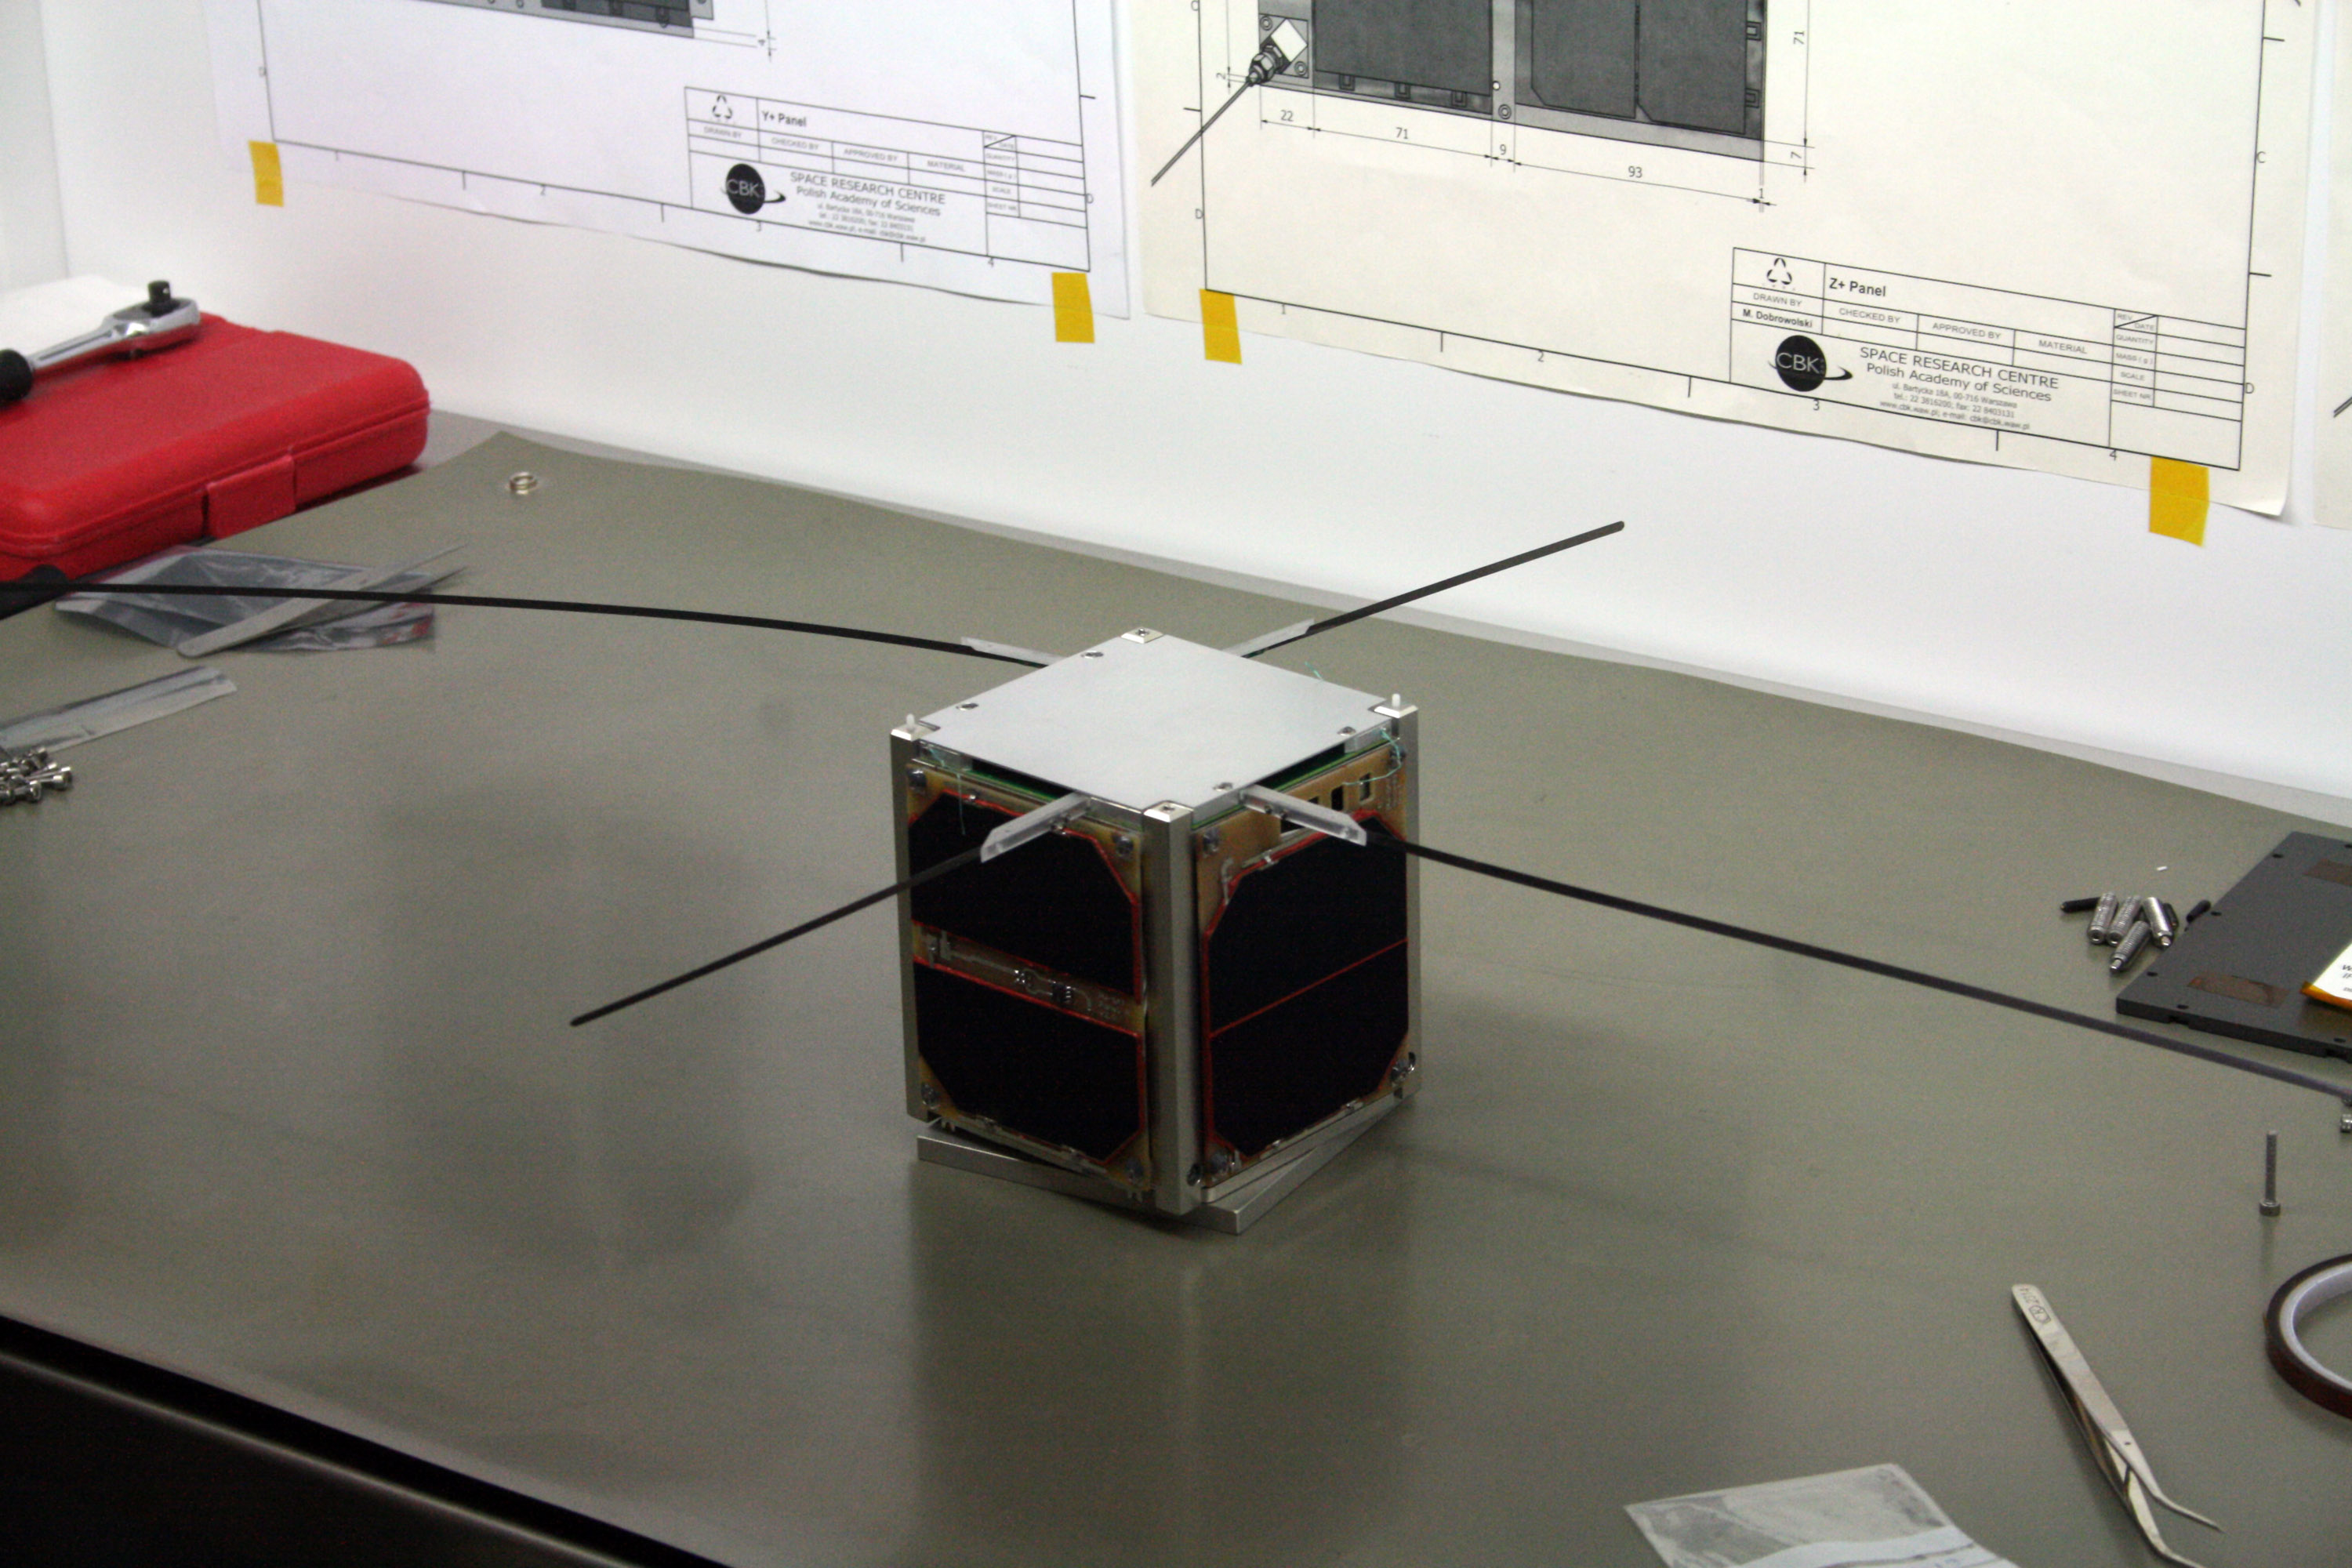
\includegraphics[width=0.32\paperwidth]{img/2/pw-sat1.jpg}
            \caption{PW-Sat1. Source: \cite{pwsat1_website_ska}}
            \label{PW-Sat1_pic}
        \end{figure}
    \end{minipage}
\end{minipage}

\subsection{SwissCube}
SwissCube is the first Swiss satellite, launched in 2009. SwissCube is 1U CubeSat, with two monopole antennas (VHF + UHF) rolled on one panel and deployed on-orbit. Housekeeping data downlink (basic telemetry) use constant \si{10}~WPM Morse code, with \SI{120}{\milli\watt} output power at \SI{437}{\MHz}. Full operational data is sent using \SI{1}{\watt} FSK modulation, \SI{1200}{\bps}. Uplink use FM-modulated AFSK signal on VHF. 

SwissCube use two Ground Stations, one at EPFL, and one at HE-Fribourg. The HE-Fribourg ground station uplink has \SI{11.4}{\dBi} of antenna-gain (one crossed \si{9}-element yagi). The downlink has \SI{14.5}{\dBi} of antenna gain (one crossed \si{17}-element yagi). The second ground station is located at EPFL in Lausanne. The performances of the EPFL ground station are slightly higher than the performances of the Fribourg ground station as there are \si{4} \si{70}-cm yagi antennas in reception (\SI{20.4}{\dBi} gain) and \si{2} \si{2}-m yagi antennas in emission (\SI{13}{\dBi} gain). \cite{swisscube_groundstation}

\begin{minipage}{\linewidth}
    \centering
    \begin{minipage}{0.45\linewidth}
        \begin{figure}[H]
            \centering
            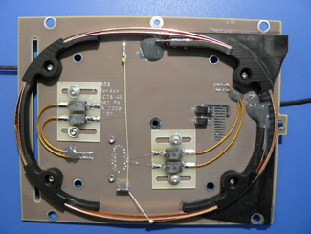
\includegraphics[width=0.32\paperwidth]{img/2/swisscube_stowed.png}
            \caption{SwissCube antennas in the stowed configuration. Source: \cite{swisscube_stowed}}
            \label{swisscube_stowed}
        \end{figure}
    \end{minipage}
    \hspace{0.05\linewidth}
    \begin{minipage}{0.45\linewidth}
        \begin{figure}[H]
            \centering
            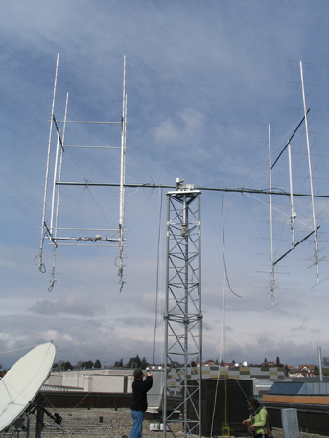
\includegraphics[width=0.32\paperwidth]{img/2/swisscube_groundstation.png}
            \caption{SwissCube EPFL ground station antennas. Source: \cite{swisscube_groundstation}}
            \label{PW-swisscube_groundstation}
        \end{figure}
    \end{minipage}
\end{minipage}
\marker[timetimetime-2-review]

%\chapter{System design}

%In this chapter, design of the radio link and component selection are described. During the design process, multiple iteration of component selection, validation and link budget calculation were made, this chapter describes the final result of the design.

\chapter{System requirements}
\section{Communication sessions}
PW-Sat2 was designed to be deployed on \SI{600}{\kilo\meter}, Sun-synchronous, polar orbit. Due to the Earts rotation, ground station coverage is bounded, and communication with the satellite is limited to communication session during satellite overpass.

Simulations performed using Gpredict software \cite{gpredict_website} shown that communication sessions will happen \si{5}-\si{6} times per day, \si{5}-\SI{10}{\minute} each. This summarizes to the total communication time to average \SI{30}{\minute} per day. Typical radio coverage of the satellite is shown in the figure \ref{gpredict_pass}.

\begin{figure}
    \centering
    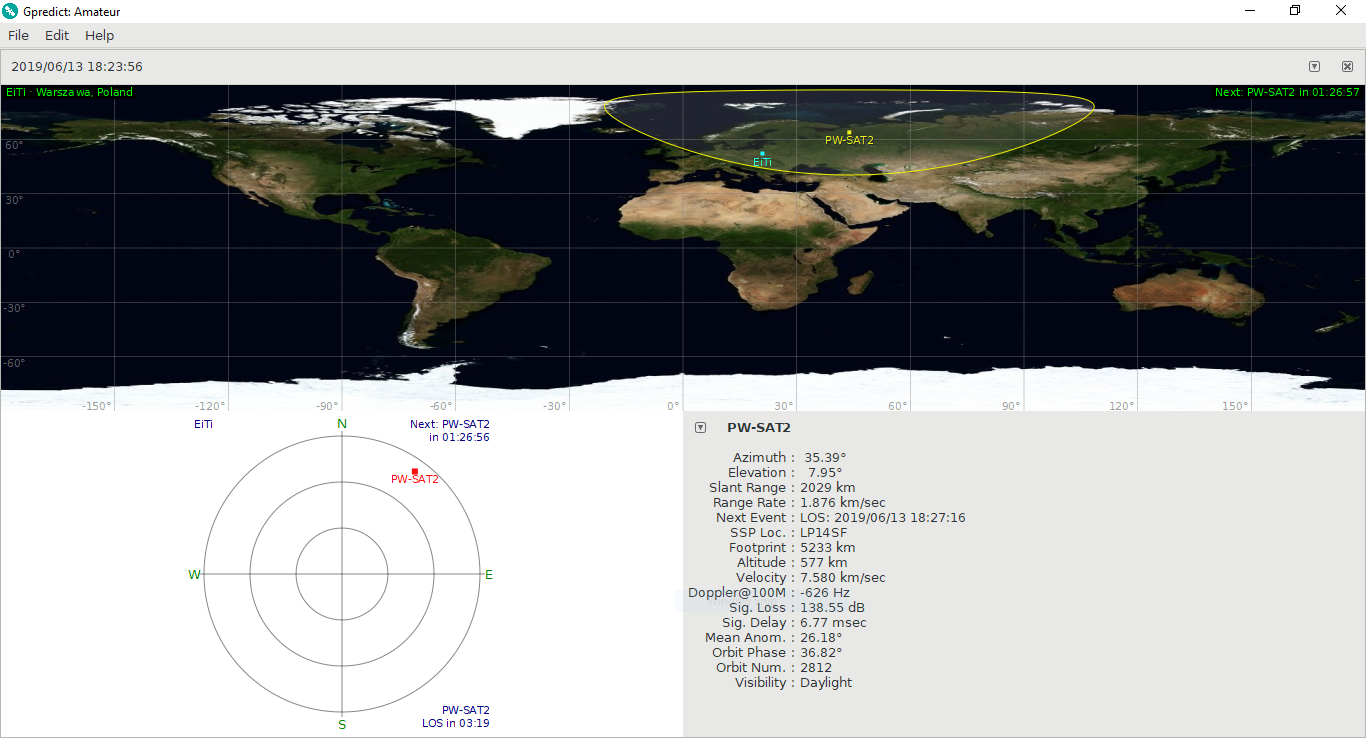
\includegraphics[width=0.8\paperwidth]{img/3/gpredict_pass.png}
    \caption{PW-Sat2 pass in Gpredict software.}
    \label{gpredict_pass}
\end{figure}


\section{Data link budget}
PW-Sat2 have couple of data sources to be sent to the ground, and each of them needs to be taken into account for estimating the required transmission throughput. For each data source the average throughput during ground station coverage is calculated, assuming \SI{30}{\minute} contact per day.
\begin{itemize}
    \item housekeeping telemetry (satellite health information, such as temperatures, bus and solar panel voltages and currents, subsystem status etc. Telemetry is \SI{230}{\byte} frame and should be transmitted every \SI{1}{\minute} (average \SI{30}{\bps}),
    \item archival housekeeping telemetry (gathered during orbit, when no ground station is in range), telemetry should be downloaded in \SI{5}{\minute} step from the whole operational time, which sums up to \SI{64}{\kilo\byte} per day (average \SI{300}{\bps}),
    \item experiment data, which are started by the operator from the ground and each of them is planned to run once a week (Sun Sensor -  \SI{32}{\kilo\byte}, RadFET - \SI{4}{\kilo\byte}, Cameras (10 photos) - \SI{300}{\kilo\byte}) - it sums up to \SI{336}{\kilo\byte} per week, average of \SI{220}{\bps},
    \item Sail deployment procedure, which transmits experiment data on-line (during the experiment). Estimated data to be transmitted (sail deployment indicator, photos and gyroscopes) is about \SI{1}{\kbps}.
\end{itemize}

Data downlink throughput requirement for PW-Sat2 mission sums up to about \SI{1}{\kbps}.
For uplink, the telecommands sent from the ground are relatively short (less than \SI{200}{\byte} each) and the rate of thelecommands is low. Therefore, no specific requirement was created, with minimal usable rate of about \SI{100}{\bps}.

\section{Frequency band selection}



\section{Communication link parameters}
Selected satellite radio module (as described in \autoref{section:comm_design}) imposes the modulation and data packets used in the communication. This section briefly describes used modulations, frame formats and implications to the ground segment of the system.

\subsection{Downlink modulation}
Downlink signal is modulated using Binary Phase Shift Keying (BPSK). The data rate can be changed dynamically by the spacecraft On-Board Computer, in range \si{1.2} - \SI{9.6}{\kbps}, allowing to improve the link quality when necessary. Baseband signal is also filtered using Raised Root Cosine filter, to reduce side lobes power. Signal bandwidth varies between \SI{2.4}{\kHz} (for \SI{1.2}{\kbps}) and \SI{19.2}{\kHz} (for \SI{9.6}{\kbps}).

% TODO: rysunek BPSK

\subsection{Uplink}
Uplink modulation is two-staged: first, data is modulated using Frequency Shift Keying with Bell 202 modem tones (0s and 1s translated to tones \SI{1200}{\hertz} and \SI{2200}{\hertz}), later to be Frequency Modulated on the RF carrier (with frequency deviation of $\pm\SI{5}{\kilo\hertz}$).

% TODO: schemat modulatora

\subsection{Frame format}
Physical layer data format is reduced-functionality AX.25 packet \cite{AX25_standard}. Only connectionless transmission mode and UI frames are supported. Packet framing is the same as in SwissCube CubeSat \cite{SwissCube_AX25}.

Basic frame format is shown in the table \ref{AX25_frame}. All the fields except flags are bit-stuffed to ensure that the \textit{Flag} field does not appear in the data: if there are six '1' bits to be send, transmitter inserts '0' bit before the last one. Adressing in this system in inherent, but unused - this is point-to-point connection, therefore adresses are fixed. Frame-Check Sequence is a CRC (CITT standard) of the whole frame (without \textit{Flags}). \textit{Information Field} is variable-length, between \si{4} and \SI{256}{\byte} length is the place for the actual data transmitted by the On-Board Computer.

\begin{table}
\small
\centering
\caption{AX.25 frame format}
\label{AX25_frame}
\arrayrulecolor{black}
\begin{tabular}{l|c|c|c|c|c|c|c|c|} 
\hhline{~|-|----|-|-|-|}
\multirow{2}{*}{}                                                              & \multirow{2}{*}{Flag } & \multicolumn{4}{c|}{AX.25 Transfer Frame Header (128 bits)}                                                                                                                                                                                   & {\cellcolor[rgb]{0.753,0.753,0.753}}                                                                                                                  & \multirow{2}{*}{\begin{tabular}[c]{@{}c@{}}Frame-\\Check\\Sequence\end{tabular}} & \multirow{2}{*}{Flag}  \\ 
\hhline{~|~|-|-|-|-|>{\arrayrulecolor[rgb]{0.753,0.753,0.753}}->{\arrayrulecolor{black}}|~|~|}
                                                                               &                        & \begin{tabular}[c]{@{}c@{}}Destination\\Address\end{tabular} & \begin{tabular}[c]{@{}c@{}}Source\\Address\end{tabular} & \begin{tabular}[c]{@{}c@{}}Control\\Bits\end{tabular} & \begin{tabular}[c]{@{}c@{}}Protocol\\Identifier\end{tabular} & \multirow{-2}{*}{{\cellcolor[rgb]{0.753,0.753,0.753}}\begin{tabular}[c]{@{}>{\cellcolor[rgb]{0.753,0.753,0.753}}c@{}}Information\\Field\end{tabular}} &                                                                                  &                        \\ 
\hline
\multicolumn{1}{|c|}{\begin{tabular}[c]{@{}c@{}}Length\\{[}bits]\end{tabular}} & 8                      & 56                                                           & 56                                                      & 8                                                     & 8                                                            & {\cellcolor[rgb]{0.753,0.753,0.753}}32-2048                                                                                                           & 16                                                                               & 8                      \\ 
\hline
\multicolumn{1}{|c|}{Value}                                                    & 01111110               & PWSAT2-0                                                     & PWSAT2-0                                                & 00000011                                              & 11110000                                                     & {\cellcolor[rgb]{0.753,0.753,0.753}}                                                                                                                  & CRC-CITT                                                                         & 01111110               \\
\hline
\end{tabular}
\end{table}


Additionally, downlink data is scrambled using G3RUH scrambling polynomial to maximize randomness and ensure proper bit synchronization.

% \marker[timetimetime-3-requirements]

% \subsection{Flatsat}

% Most of the tests were performed on Flatsat (an abbreviation from Flat Satellite), an electronic test bench, which consist of mix of flight models, engineering models of the instruments and Electrical Ground Support Equipment (EGSE). EGSE are the test instruments and/or mocks (fake) instruments, which allow testing without the need for actual hardware.

% PW-Sat2 Flatsat was integrated in Space Research Centre in Warsaw. Flatsat is shown in the figure \ref{TODO}.

% \subsubsection{Flatsat Ground Station mock}
% To perform the communication tests a Ground Station mock was created of flatsat. It was built using to Software-Defined Radios: one, as downlink receiver, same as to be installed in the Ground Station (Funcube Pro+), and the second (PlutoSDR) to generate uplink signals. Use of SDR instead of analogue radio transceiver greatly simplified the tests performed. Ground station mock is shown in the figure \ref{TODO}. 




\chapter{Space segment}
Space segment is a part of the satellite communication system that resides on the satellite itself. It is divided into two main parts: communication subsystem (COMM) and antennas (ANTs) connected with two coaxial cables.

Space segment is critical in system operation and reliability - there is no possibility to carry out any repairs, perform maintenance or adjustment once on orbit. It is exposed to the space environment - wide temperature range, thermal cycling, cosmic radiation and vacuum.

Because of the mentioned requirements it was decided to choose commercially available and flight-proven CubeSat components to increase the overall reliability of the system.

% -----------------------------------------------------------------------------------------------------------
% -----------------------------------------------------------------------------------------------------------
% -----------------------------------------------------------------------------------------------------------

\section{Spacecraft communication transceiver}
\label{section:comm_design}
CubeSat design specification \cite{cubesat_spec}, with which PW-Sat2 is compliant, defines common PC/104 connector, which is the main data bus for all satellite subsystems. On the connector, two \iic and two CAN buses are defined and most of the components are compatible to each other. However, due to the lack of CAN interface on On-Board Computer (CubeComputer from CubeSpace \cite{cubespace_website}) radio should use \iic communication bus.

When the subsystem was ordered (in year \si{2014}), the choice of available products was very limited, and the only radio which was compliant with above mentioned requirements was \texttt{ISIS VHF uplink/UHF downlink Full Duplex Transceiver}. Its view and block diagram is shown in the figure \ref{ISIS_TRXvU}

\begin{figure*}
   \centering
\begin{tabular}{cc}
        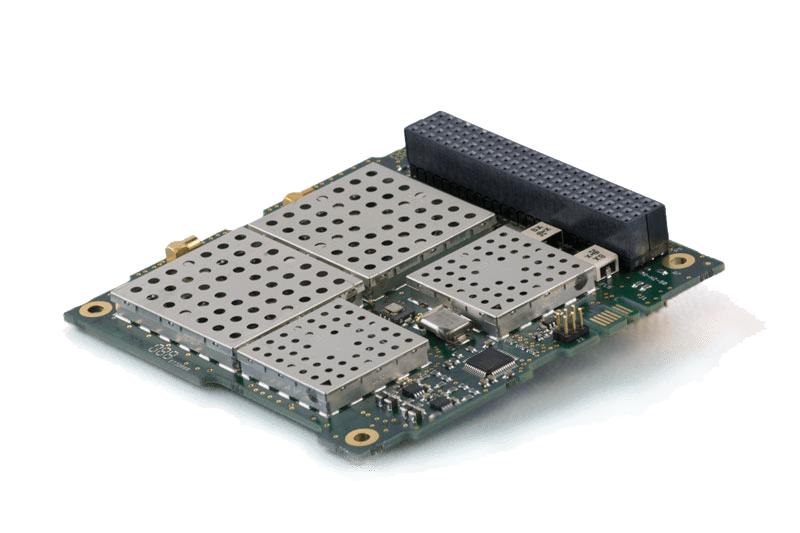
\includegraphics[width=0.3\paperwidth]{img/4/ISIS-radio-UHF-VHF-min.png}
    & 
        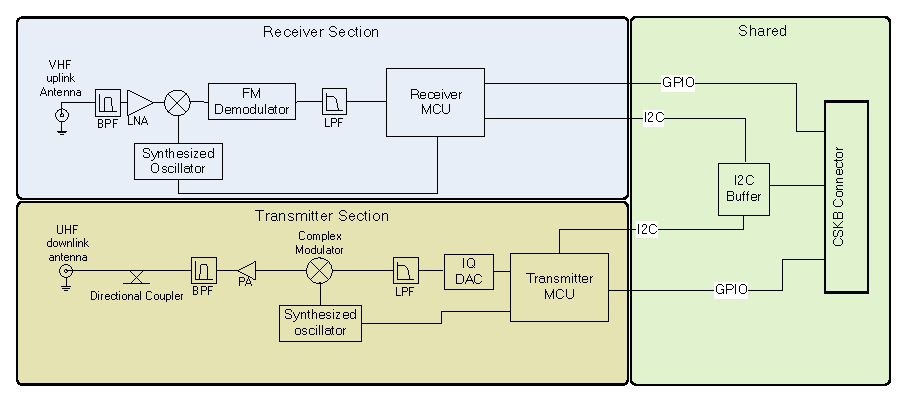
\includegraphics[width=0.4\paperwidth]{img/4/ISIS_TRXvU_block_diagram.eps}
\end{tabular}
\label{ISIS_TRXvU}
\caption{ISIS VHF uplink/UHF downlink Full Duplex Transceiver. Source: \cite{isis_trxvu}}
\end{figure*}

Basic characteristics: \\
\begin{tabular}{c|c}
     \textbf{downlink} & \textbf{uplink} \\ \hline
     \multicolumn{2}{c}{dual-\iic communication standard} \\
     \multicolumn{2}{c}{AX.25 frame format} \\
     \si{430}-\SI{450}{\MHz} frequency range & \si{140}-\SI{150}{\MHz} frequency range \\
     \SI{0.5}{\watt} downlink power & \SI{-98}{\dBm} sensitivity for \si{10^-5}~BER \\
     \si{1.2} - \SI{9.6}{\kilo\bit / \second} bitrate & \SI{1.2}{\kilo\bit / \second} bitrate \\ 
     BPSK modulation with G3RUH scrambling & FM-modulated AFSK \\ 
\end{tabular}

Transceiver was tested separately for its uplink and downlink capabilities. Tests are critical to make sure that radio parameters are maintained in the system, and to verify manufacturers' data.

\subsection{Uplink measurements}
The most important parameter of the radio receiver is the sensitivity. Blocking immunity (intermodulation), is not critical, as the system is remote from most of the external strong radio signals.

\subsubsection{Sensitivity}
Sensitivity was measured by the setup shown in the figure \ref{TODO}. Test procedure:
\begin{itemize}
    \item measuring output power of PlutoSDR using spectrum analyzer with wide RBW filter (\SI{1}{\MHz})
    \item increasing attenuation up to the point when PER is noticeable (\SI{1}{\percent})
    \item calculating signal input power
\end{itemize}

The result of this test was the sensitivity of TODO.

\subsubsection{Doppler}
Doppler effect is caused when fast-moving object is emitting/receiving radio waves. For uplink frequency (VHF band) Doppler effect influence can shift frequency up to about \SI{5}{\kHz}. The receiver bandwidth should be measured to estimate allowable frequency inaccuracies.

Test setup is the same as in previous setup, shown in the figure \ref{TODO}. During the test the PER was measured for a range of frequency shift from center. The result is shown in the chart \ref{TODO}.

\subsection{Downlink measurements}
Downlink parameters of the radio module were also measured. An important parameter is the output power and the spectrum of the signal.

\subsubsection{Output power}
Output power was measured using spectrum analyser with wide resolution bandswidth (\SI{1}{\MHz}). Output power was measured to be \SI{27}{\dBm}. TODO

\subsubsection{Spectrum}




% -----------------------------------------------------------------------------------------------------------
% -----------------------------------------------------------------------------------------------------------
% -----------------------------------------------------------------------------------------------------------



\section{Spacecraft Antennas}
Because of the selected radio system, two antennas has to be installed - one for uplink (VHF) and one for downlink (UHF). Antennas should be omnidirectional, as PW-Sat2 does not have an nadir-pointing capability and random tumbling during operation is assumed.

Self-made dipole antenna was considered at the design stage, but due to mechanical and time constraints, satellite antenna was decided to be bought as well. Innovative Solutions In Space company sells antenna with with the transceiver as CubeSat communication Kit \texttt{CubeSat dipole antenna system}. Both elements are compatibile and the whole system (transceiver + antenna) is tuned for specific communication frequency and mounting option.

This system is deployable by the command from the on-board computer. Thermal knife (resistor) is heated up and thermal link is burnt, resulting is antenna deploy by the spring action. Antenna is shown in the figure \ref{ISIS_antenna}.

\begin{figure*}
   \centering
\begin{tabular}{cc}
        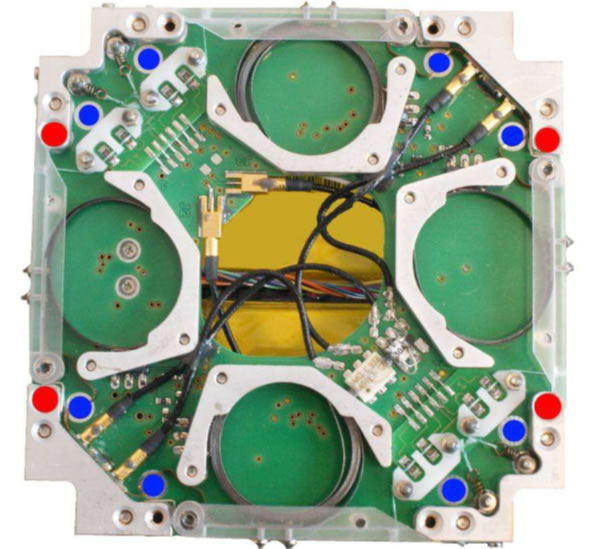
\includegraphics[width=0.3\paperwidth]{img/4/isis_antenna_stowed.jpg}
    & 
        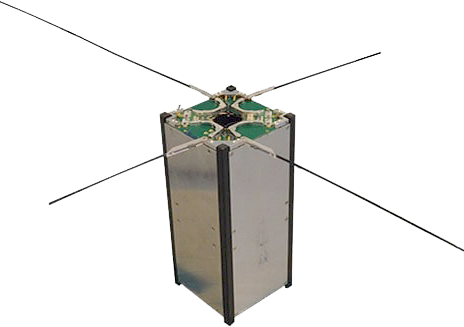
\includegraphics[width=0.45\paperwidth]{img/4/CubeSat-antenna-dipole-configuration.png}    
\end{tabular}
\label{ISIS_antenna}
\caption{ISIS CubeSat dipole antenna system in stowed and deployed position. Source: \cite{isis_dipole_antenna}}
\end{figure*}


\subsection{Measurements}
After deployment on the orbit, antennas have to deploy. During the test campaign antenna deployment procedure was executed three times. Deployed antennas are shown in the figure \ref{TODO}.

Reflected power from antenna is measured by the radio module during radio frame transmission. Correct antenna deployment can be assured by using the telemetry and comparing the reflected power with measured during the ground test campain. 
Reflected and forward power chart captured during second antenna opening are shown in the figure \ref{TODO}.

% -----------------------------------------------------------------------------------------------------------
% -----------------------------------------------------------------------------------------------------------
% -----------------------------------------------------------------------------------------------------------

% \subsubsection{Deployable elements influence on the antenna pattern}
% TODO

% On-board PW-Sat2 are two main deployables: solar panels and deorbitation sail.

% During design stage, influence of the solar panels was discussed with antenna manufacturer - the outcome was to place longed dipoles (VHF) along the solar panels, and shorter ones orthogonally to it, as shown in the figure \ref{???}

% % TODO: zdjęcie z otwartymi panelami i antenami

% The influence of the deorbit sail was also simulated during Critical Design stage.

% Deorbitation sail is made by very thin (\SI{5}{\micro\meter}) mylar foil with aluminium coating. Using % TODO
% simulation tool, it was shown that the sail will increase directivity of the cubesat antennas, acting as a reflector.
% % TODO: jakieś zdjęcie z symulacji, wynik o ile dB się pogorszyło



\marker[timetimetime-4-space]

\chapter{Ground segment}
Ground station design should complement the space segment, with large antenna gains and output power to allow the budget link to close. As the system is full-duplex, both uplink and downlink channels are separate and the design should allow to simultaneously operate transmit and receive. Block diagram of the designed ground station is shown in the figure \ref{gs_block_diagram}.
Due to the low sensitivity of the satellite receiver (\SI{-98}{\dBm}) uplink EIRP has to be very large, this is achieved by using high-power amplifier and antennas with high directional gain. For downlink, ground station has to compensate low transmit power of the satellite, by using high gain antennas and very sensitive receiver.

Ground station consists of not only the hardware but also software. Many parts of the system use Digital Signal Processing and Software-Defined Radio for data modulation/de-modulation, packet transmission etc. For the DSP tasks, GNUradio \cite{gnuradio} was selected and the tool for sampling-based signal processing.



\begin{figure}[H]
    \centering
    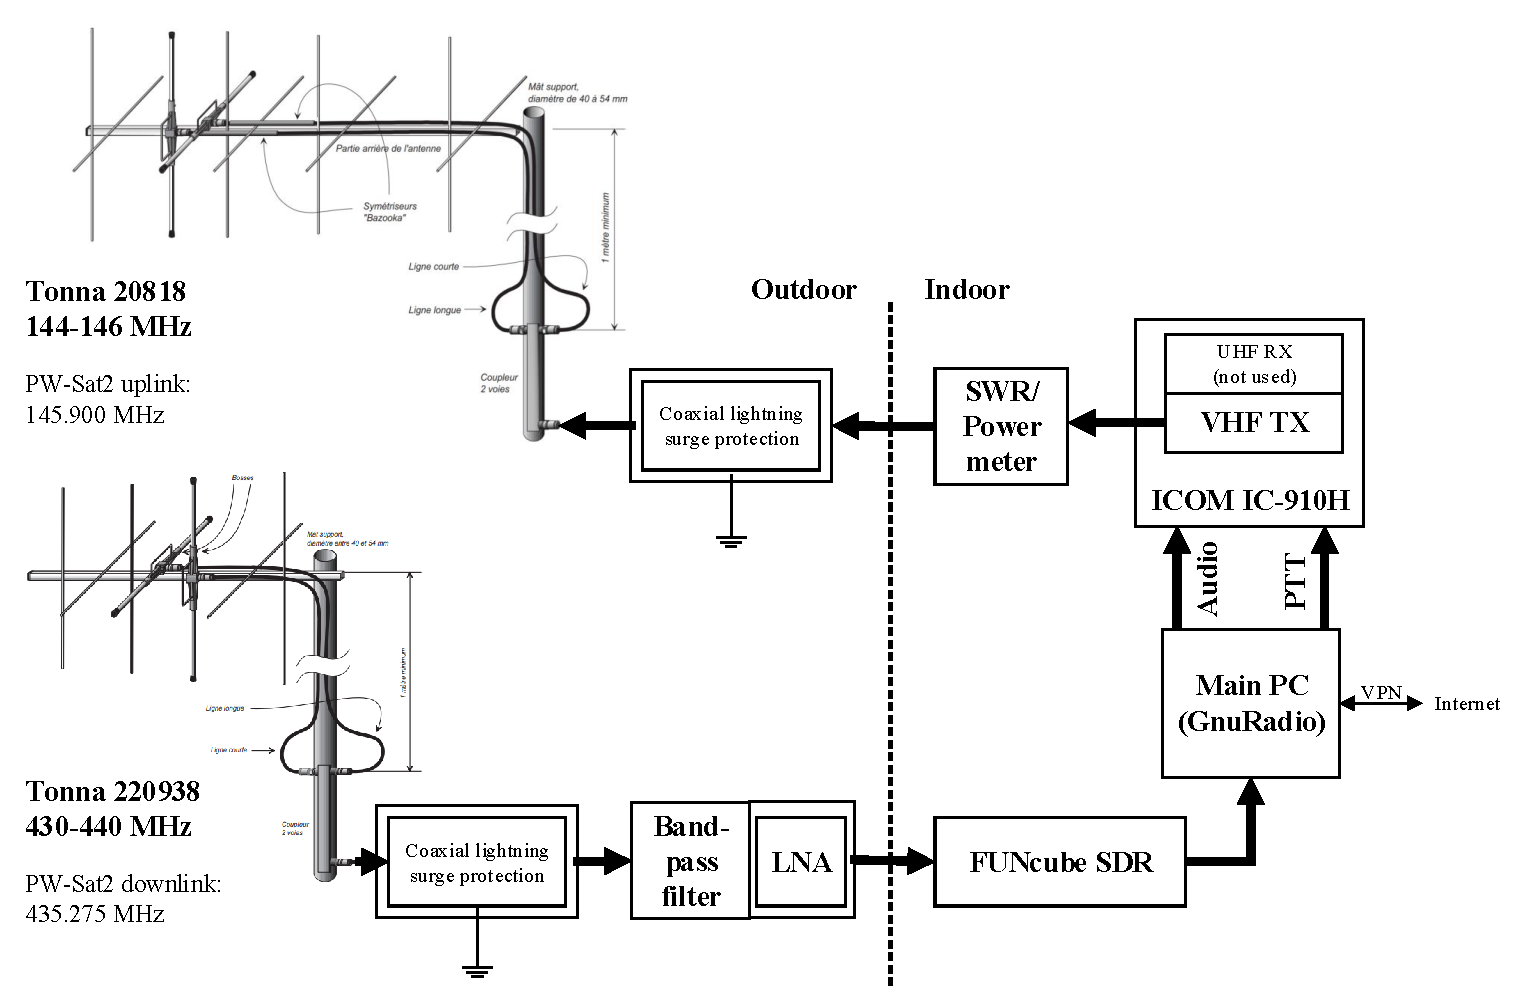
\includegraphics[width=0.8\paperwidth]{img/5/gs_block_diagram.eps}
    \caption{Ground station block diagram}
    \label{gs_block_diagram}
\end{figure}


\section{Antennas}
PW-Sat2 is transmitting radio signals with linear polarization, nevertheless ground station  polarization should be circular, due to the random tumbling of the satellite. This will reduce the gain of the antennas, but the signal strength will be constant regardless of the satellite rotation. Cross-Yagi antennas were selected, and two linear planes antennas were phased with coaxial cable and symmetrical splitters/combiners. Coaxial cables length was calculated to achieve \SI{90}{\degree} shift between two dipoles.

Antennas were selected to be the longest possible, limited by the antenna mast height. Selected antenna characteristics:

\begin{tabular}{c|c}
     \textbf{Downlink} & \textbf{Uplink} \\ \hline
     Tonna 220938 & Tonna 20818 \\
     2x 19 elements & 2x 9 elements \\
     loop dipole & linear dipole \\
     \SI{16.2}{\dBi} gain & \SI{13.2}{\dBi} gain \\
     \SI{30}{\degree} beamwidth & \SI{40}{\degree} beamwidth
\end{tabular}

Additionally, two combiners were selected for antenna phasing: Tonna 31202 for VHF and Tonna 31270 for UHF. Antennas are also protected by the Coaxial lightning surge protection, to minimise risk of damaging indoor equipment.

\subsection{Measurements}
After the assembly, antennas should be measured to make sure of the correct assembly. The simplest method is to measure the impedance of the antennas.

Each antenna consist of two dipoles (with vertical and horizontal polarization) phased with a combiner. Measurements of the dipoles and the phased antenna were performed, and the result is shown in the table \ref{TODO}.


\section{Uplink - transmitter}
Uplink signal is an FM-modulated AFSK, so standard analog audio FM transceiver can be used to generate RF signal. The frequency deviation of the de-modulator was selected to allow to use radio amateur voice transceivers. Audio signal (before FM-modulation) is generated by the software running on the PC.

During PW-Sat1 project, the Icom 910H amateur radio transceiver was used for both uplink and downlink, therefore it was proposed to use the the same radio as it do comply with all the requirements. Radio is shown in the figure \ref{Icom_910H_ref}.

\begin{figure}[H]
    \centering
    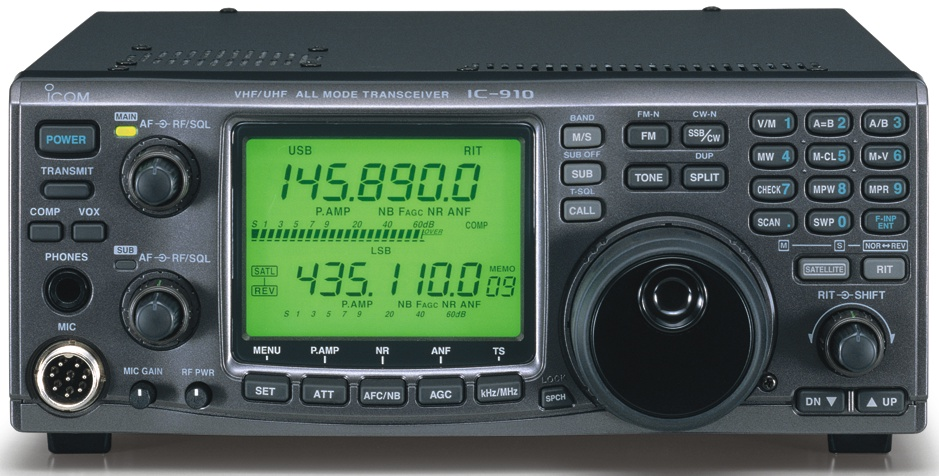
\includegraphics[width=0.6\paperwidth]{img/5/icom910h.jpg}
    \caption{Icom 910H. Source: \cite{ICOM_910H_pic}}
    \label{Icom_910H_ref}
\end{figure}

Radio VHF FM transmit characteristics:

\begin{tabular}{c|c}
    Frequency & \si{144} - \SI{148}{\MHz} \\
    Frequency stability &  \SI{\pm 3}{\ppm} \\
    Output power & \SI{100}{\watt} \\
    Audio input & analog jack \\
    Audio bandwidth & \SI{4}{\kHz} \\
\end{tabular}

\subsection{Data flow}
This radio is connected to the computer, which controls the audio to transmit and Push-To-Talk (PTT, transmission enable) signal. Uplink baseband signal (AFSK) has generated by the GNURadio framework, to be later FM-modulated and transmitted using conventional radio. Block diagram of uplink data chain is shown in the figure \ref{uplink_data_flow}

\begin{figure}[H]
    \centering
    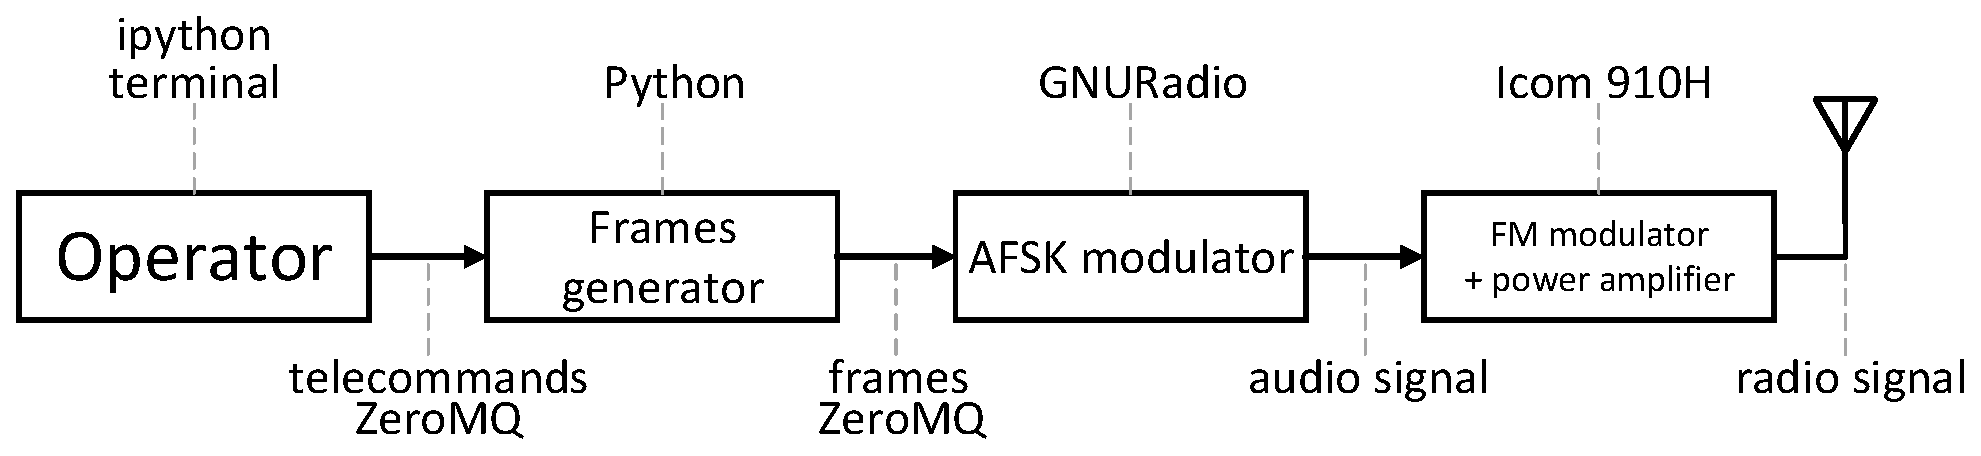
\includegraphics[width=0.6\paperwidth]{img/5/uplink_data_flow.eps}
    \caption{Uplink data flow}
    \label{uplink_data_flow}
\end{figure}

AFSK signal generation GNURadio flowgraph is shown in the figure \ref{uplink_flowgraph}. Audio signal is generated by software Voltage Controlled Oscillator (VCO), and the frequency is controlled by the actual bit value (\SI{1200}{\hertz} or \SI{2200}{\hertz}).

% TODO: uplink_flowgraph


\subsection{Standing Wave Ratio meter}
To check proper antenna connection and ensure long-term monitoring a SWR (Standing Wave Ratio) was installed. This instrument measures ratio of reflected power, thus providing information about antenna impedance matching. In case of antenna break

% TODO: zdjęcie/zrzut z kamerki SWR metera


\subsection{Measurements}
As the uplink was built using conventional HAM radio transceiver, only the modulation and output power should be measured. As the physical layer is the typical FM-modulated AFSK and frame protocol is typical AX.25 there is a lot of free software to verify the correctness of the frame and modulation.

\subsubsection{Output power}
The power of the power amplifier (built in the transceiver) was measured using an SWR \& Power Meter TODO, and by connecting radio output to the antenna. The measured output and SWR was equal to TODO. Those parameters are continuously monitored during the mission to monitor the cables and radio health.

\subsubsection{Spectrum \& Watchdogs}
The spectrum and output modulation correctness in constantly monitored using so-called watchdogs built using another Software Defined Radios (PlutoSDR, RTL-SDR) placed in the proximity of the main antennas.
By demodulating uplink signal and comparing it in the real time with transmitted frames the correctness of the transmission is guaranteed. Watchdog flowchart and graphical view are shown in the figure \ref{TODO}.



% ------------------------------------------------------------
% ------------------------- DOWNLINK -------------------------
% ------------------------------------------------------------

\section{Downlink}
Receiving Signals from maximal slant range of about \SI{3000}{\kilo\meter} from a \SI{0.5}{\watt} transmitter requires very high processing gain and low noise factor of the system. System also needs to compensate for Doppler effect and ground interferences.

\subsection{Signal front-end processing}
Radio front-end has two main purposes - to lower the system noise figure (by amplifying the signal with Low Noise Amplifier) and eliminate intermodulation with another signals (filtering). Low Noise Amplifier, installed close to the antenna reduces influence of the long cable to the receiver and reduces the noise added by receiver, reducing total system noise factor. Noise factor is limited by the attenuation between the antenna and Low Noise Amplifier and the Noise Factor of the amplifier itself. However, strong signals in the frequency proximity of the signal can intermodulate in the LNA, resulting in variety of issues: from reduced gain to completely distorted signal.

Narrow-band filter should be installed before the LNA. However, this requires the filter to have the lower loss possible, as the insertion loss of the filter directly affects noise figure of the system. For this purpose, cavity filter was selected. This, narrow band filter (\SI{1}{\MHz}), has very low insertion loss as shown in the measurement chapter. After the filter, Low Noise Amplifier is mounted.

Front-end signal processing is installed as close to the antenna as possible as shown in the figure \ref{elka_skrzynka}.

\begin{figure*}
   \centering
\begin{tabular}{cc}
        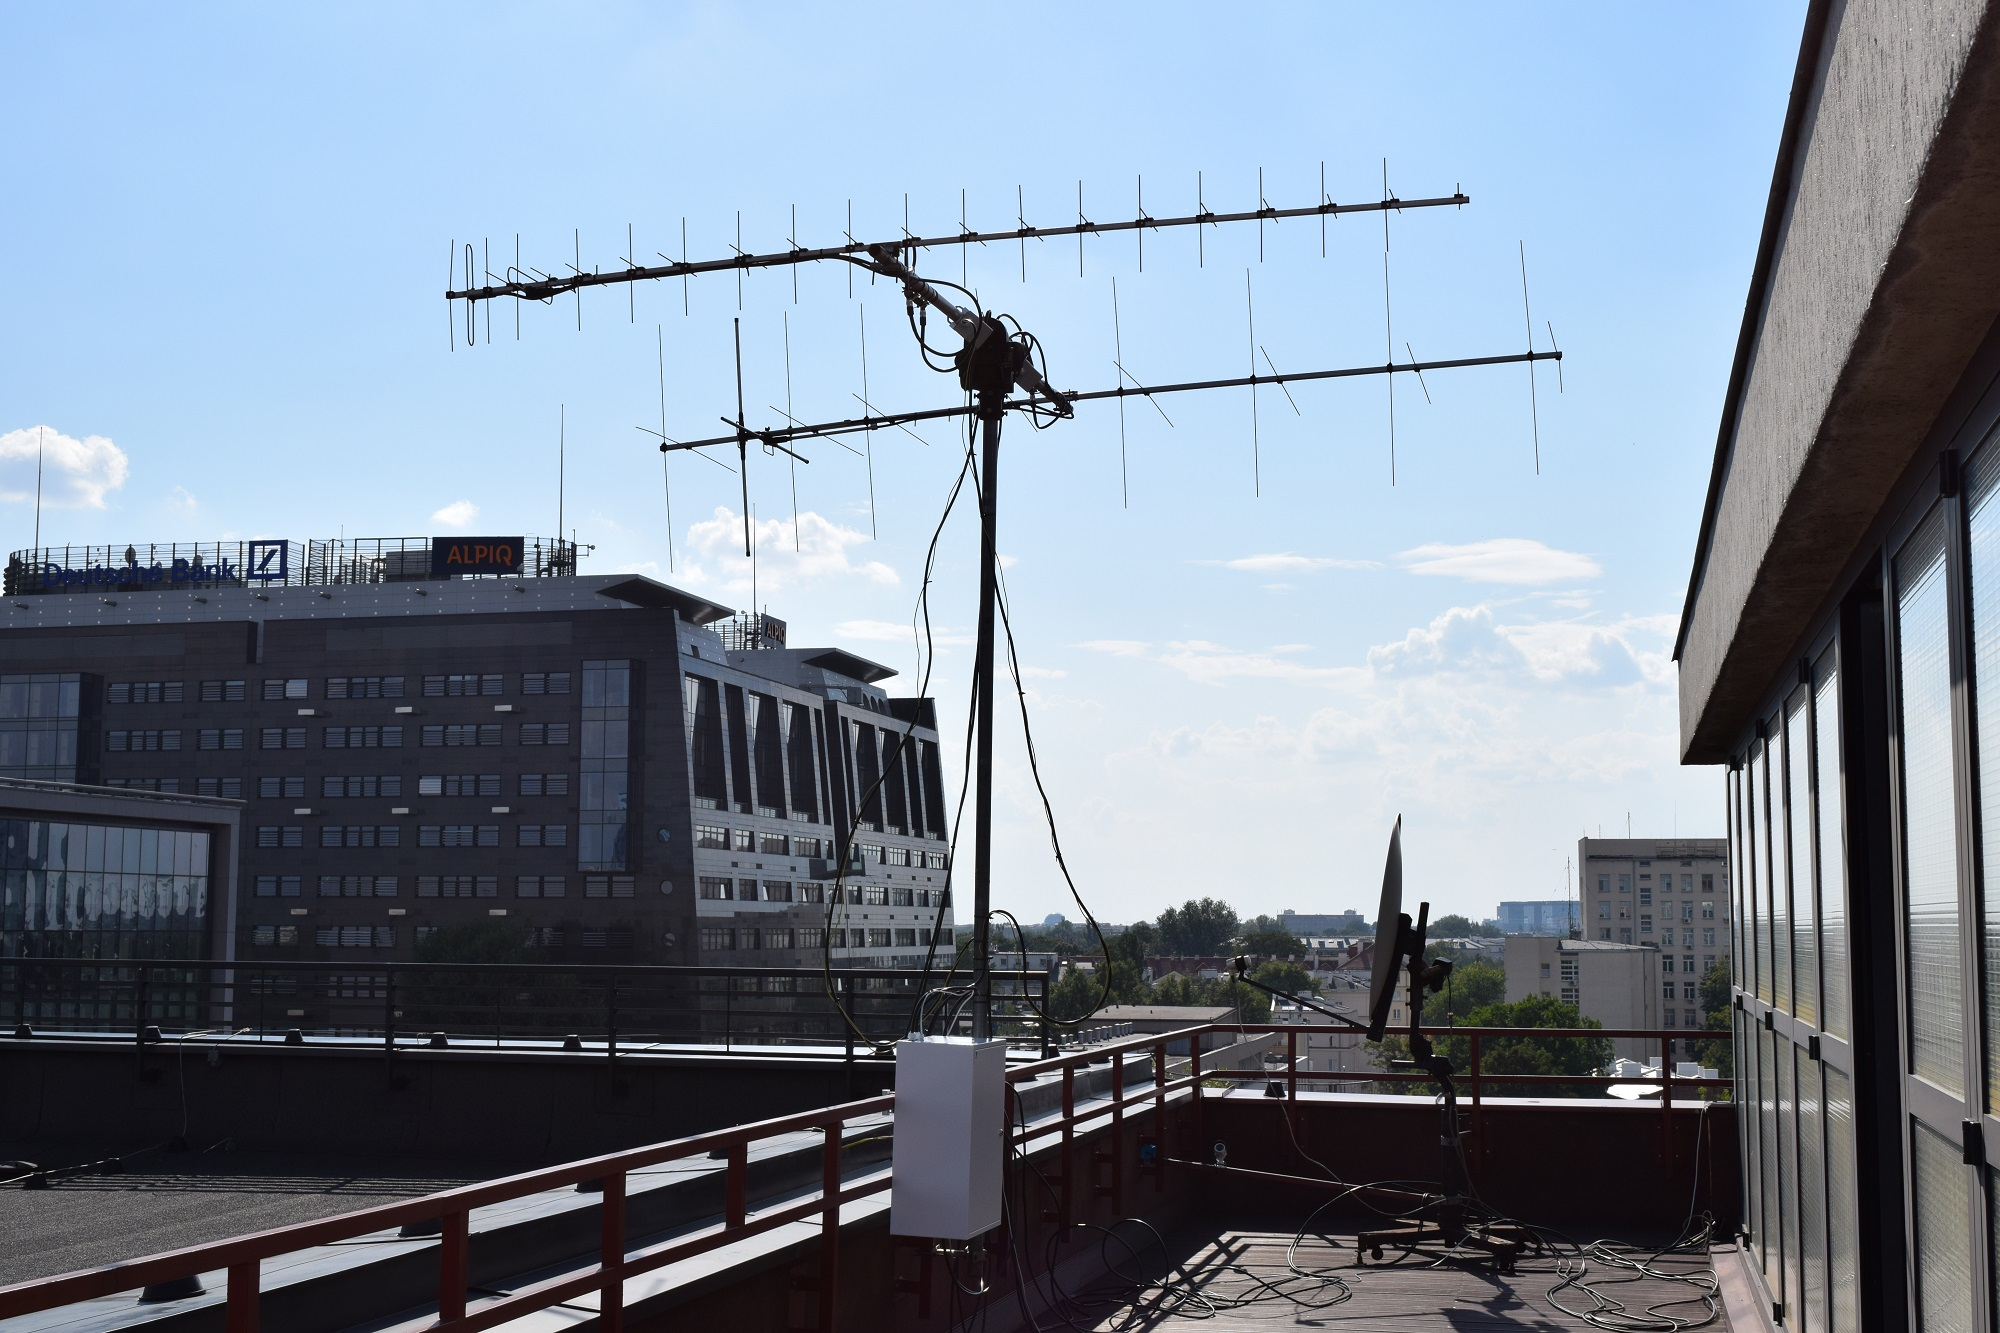
\includegraphics[width=0.3\paperwidth]{img/5/elka_view.jpg}
    & 
        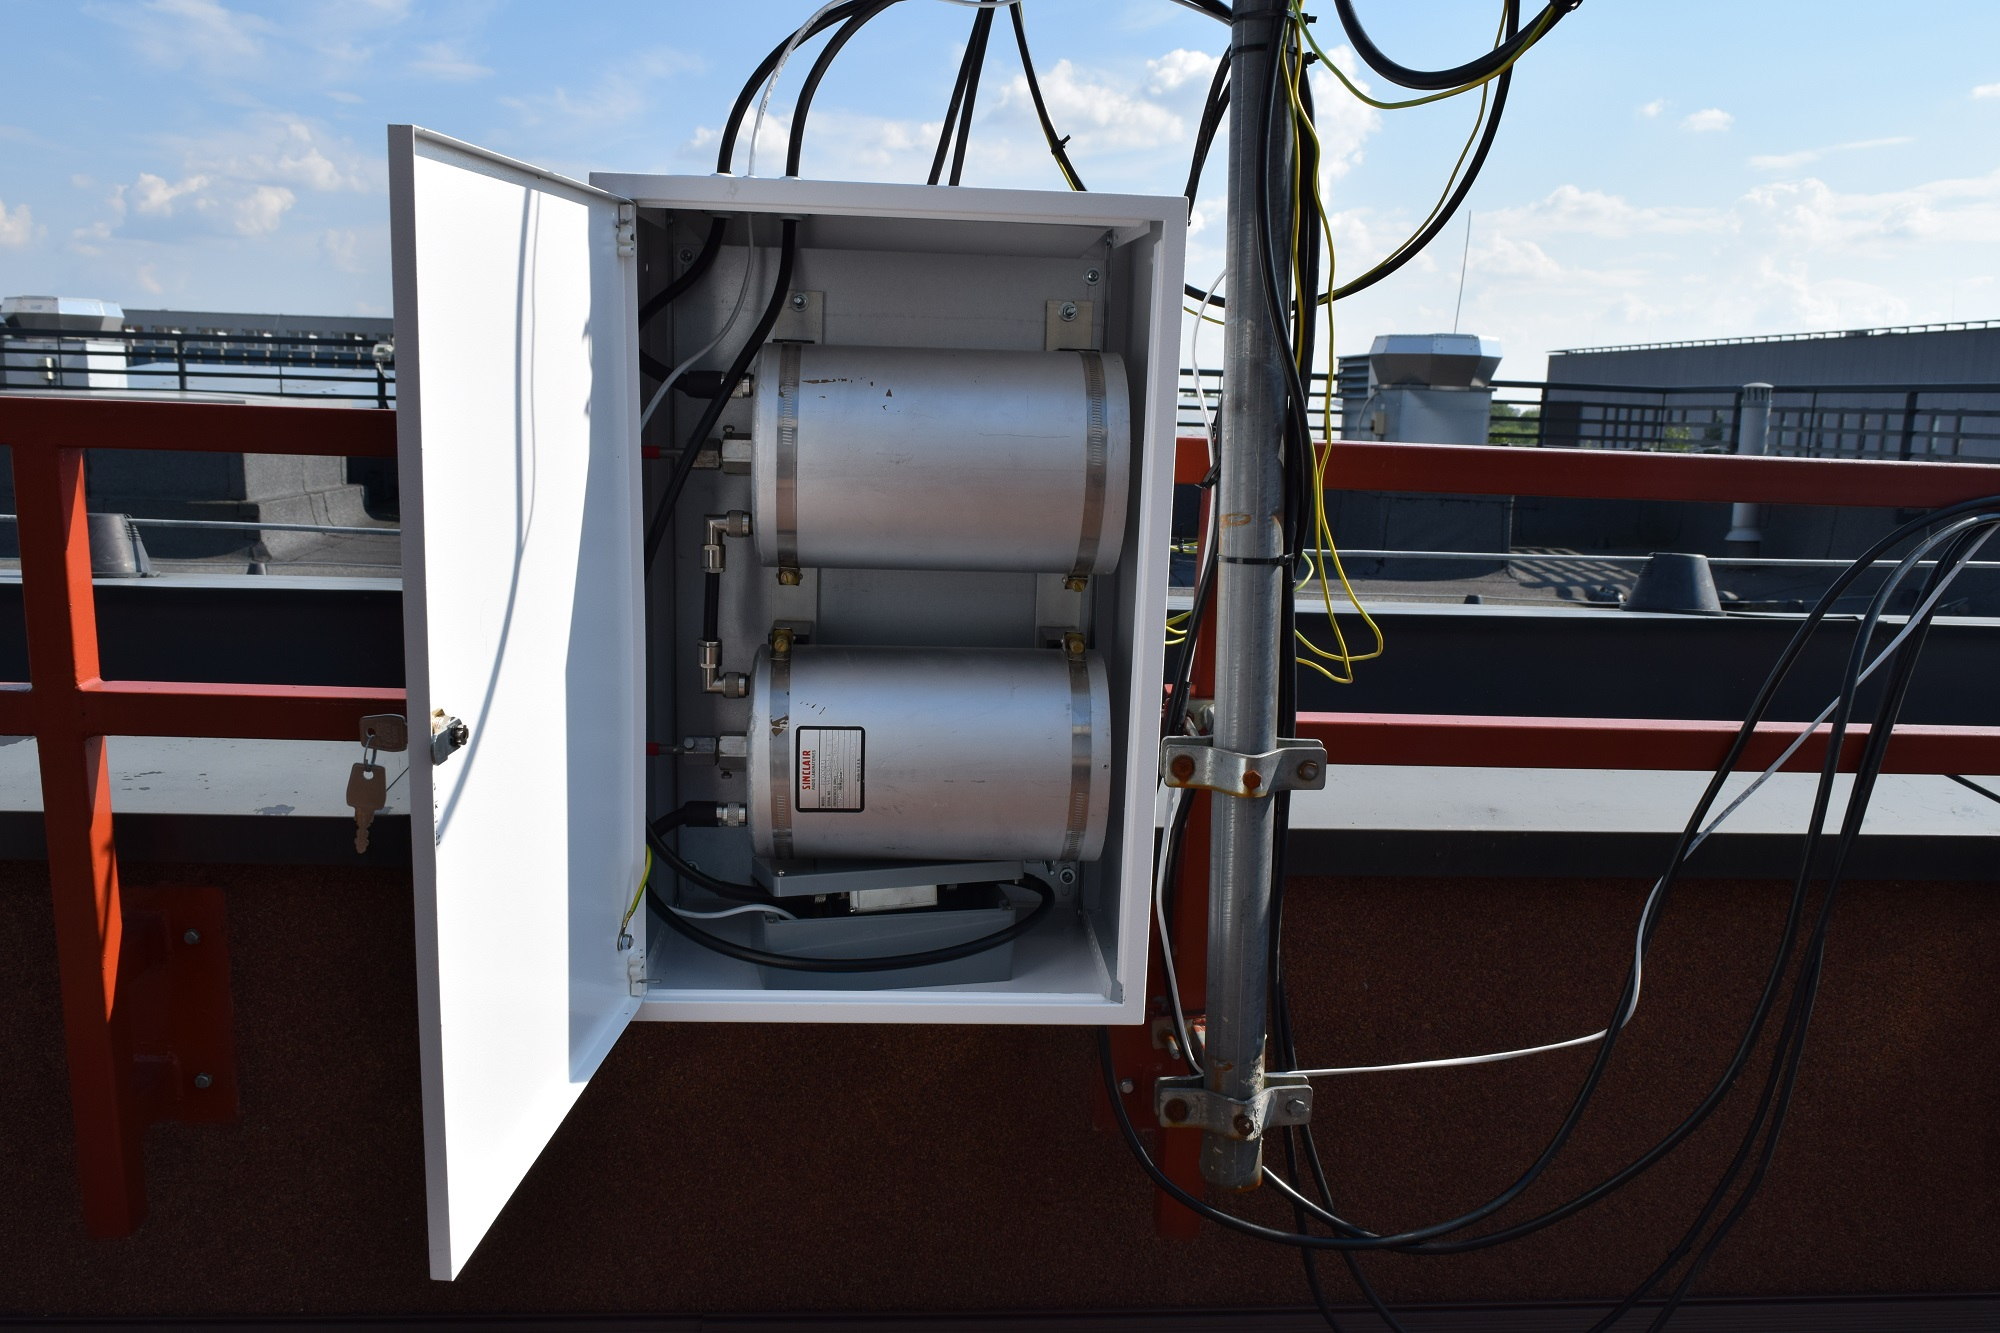
\includegraphics[width=0.3\paperwidth]{img/5/elka_skrzynka.jpg}
\end{tabular}
\label{elka_skrzynka}
\caption{PW-Sat2 ground station view and front-end processing.}
\end{figure*}

\subsubsection{Filter measurements}
Cavity filter was tuned to the required frequency to minimize insertion loss and bandwidth. Signal bandwidth is very narrow compared to the filter frequency range.
The insertion loss and band pass range was measured using Network Analyser. S-parameters are shown in the figure \ref{TODO} and the filter parameters are summarised in the table \ref{TODO}.

\subsection{Low noise amplifier}
A dedicated Low Noise Amplifier was designed. It should eliminate out-of-band signals and amplify the required downlink frequency by at least \SI{20}{\dB}. As the main active component, a high-level Low Noise Amplifier: Mini-Circuits PGA-103+ \cite{lna_pga_datasheet} was used. Additional \SI{433}{\MHz} SAW filter was placed before the amplifier to reduce out of band interferences signals. Bias of the amplifier is created by RF Low Dropout Regulator Texas Instruments TPS7A47 \cite{lna_ldo_datasheet}. Amplifier was designed to support two-stage configuration, but for PW-Sat2 only first stage was populated. Schematic, PCD layout and the picture of the designed board are shown in the figures: \ref{lna_schematic} and \ref{lna_pcb}. The design is open source and all the source files can be found at \cite{lna_github}

\begin{figure}[H]
    \centering
    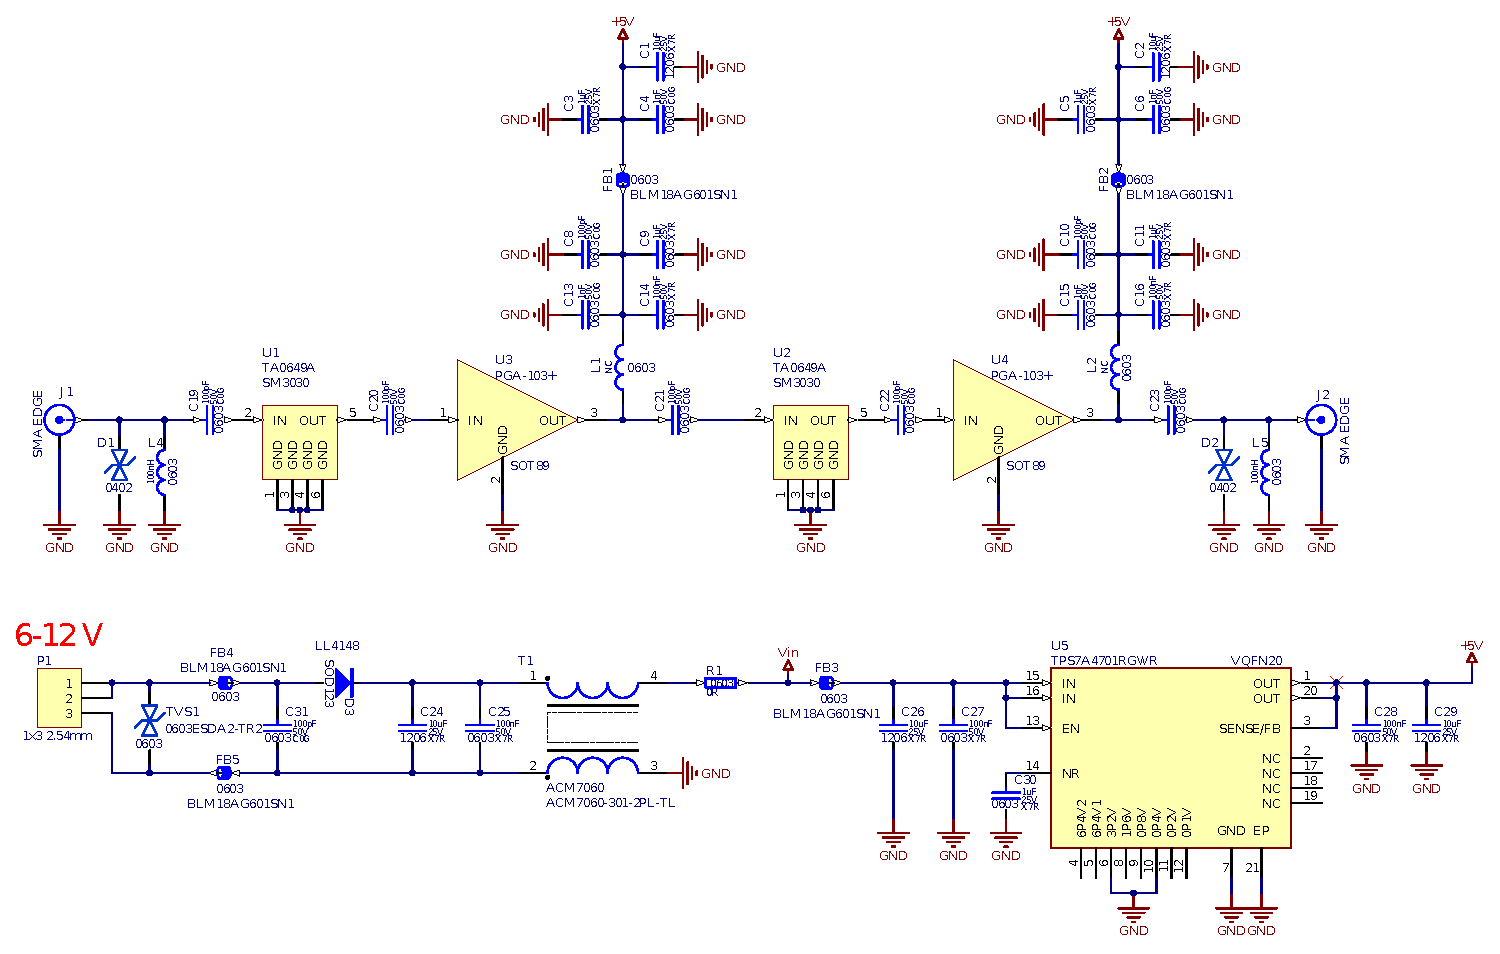
\includegraphics[width=0.8\paperwidth]{img/5/lna_schematic.eps}
    \caption{Low Noise Amplifier Schematic}
    \label{lna_schematic}
\end{figure}

\begin{figure*}
   \centering
\begin{tabular}{cc}
        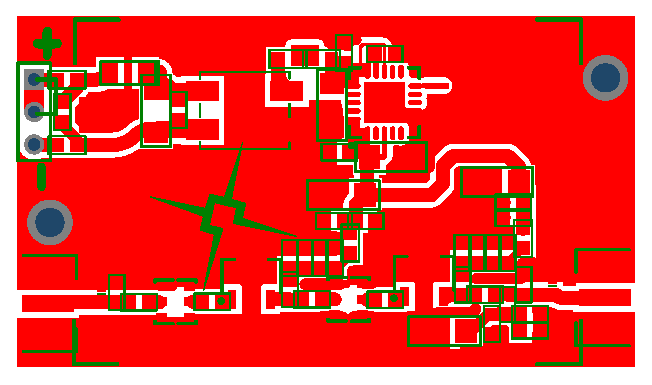
\includegraphics[width=0.4\paperwidth]{img/5/lna_pcb.eps}
    & 
        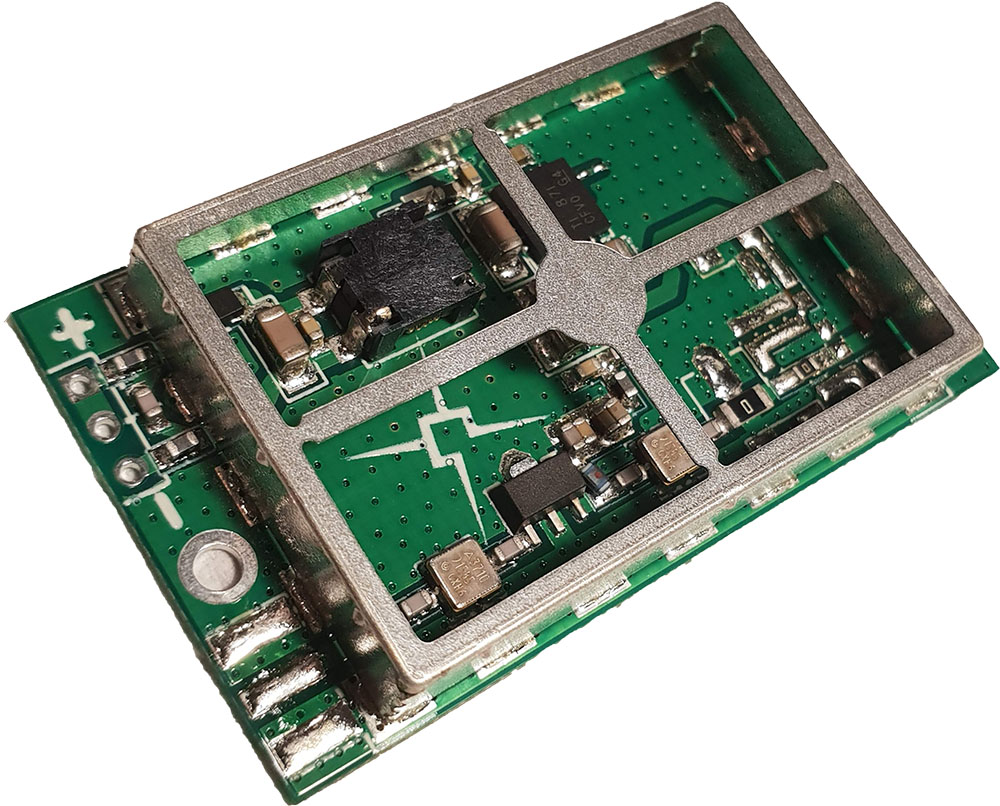
\includegraphics[width=0.3\paperwidth]{img/5/lna_assembled.jpg}
\end{tabular}
\label{lna_pcb}
\caption{Low Noise Amplifier PCB layout and assembled picture}
\end{figure*}


\subsubsection{Measurements}
Designed Low Noise Amplifier is shown in the figure \ref{TODO}. Its S-parameters were tested using Rohde\& Schwarz ZVL. Results are shown in the figure \ref{TODO}. Gain and frequency were as expected and are shown in the table \ref{TODO}.


\subsection{Receiver}
Due to the custom packet format no commercially available integrated circuits were able to correctly receive packets, therefore a custom solution was required for de-modulation and packet recovery.
To receive BPSK signals, the phase recovery is necessary. One of the methods of the synchronous detection is the use of Costas loop \cite{costas_loop}. Most simple solution is to implement full signal chain: Costas loop, bit recovery and packet formatting into software, therefore requiring down-conversion of the signal and data transfer to the PC. 

One of the possible and widely used methods is to use radio amateur transceiver in SSB mode - then radio acts as a multi-stage down-converter, allowing to receive baseband with audio card from PC. However, due to main purpose of transmitting audio signals, there is a lowpass filter for baseband at about \SI{3}{\kHz}. Using SSB mode for receiving PW-Sat2 is possible, however only for \SI{1.2}{\kbps} bitrate.

Another method was to use Software-Defined Radio, performing IQ downconversion and data transmission. The Radio Amateur Satellite Corporation designed an SDR receiver for their mission FUNcube Satellite. After mission success, they released their design and started selling FUNcube dongle shown in the figure \ref{funcube_pic}. Given that is was designed specifically for satellite communication and it was tested using similar CubeSat design, it was selected as the main receiver for PW-Sat2.

\begin{figure}[H]
    \centering
    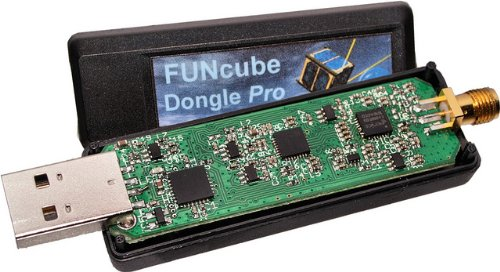
\includegraphics[width=0.6\paperwidth]{img/2/funcube.jpg}
    \caption{FUNcube Dongle Pro+. Source: \cite{funcube}}
    \label{funcube_pic}
\end{figure}

The receiver  functionalities:
\begin{itemize}
    \item Doppler correction,
    \item IQ data recording,
    \item BPSK demodulation,
    \item bit recovery,
    \item packet formatting,
    \item multiple bitrate simultaneous decoders,
    \item sending data on-line to the operators,
    \item work with different Software-Defined Radios and SSB transceivers
\end{itemize}

The block diagram of the designed system is shown in the figure \ref{demodulator_block_diagram}. All of the signal processing blocks were created using GNUradio framework.

\begin{figure}[H]
    \centering
    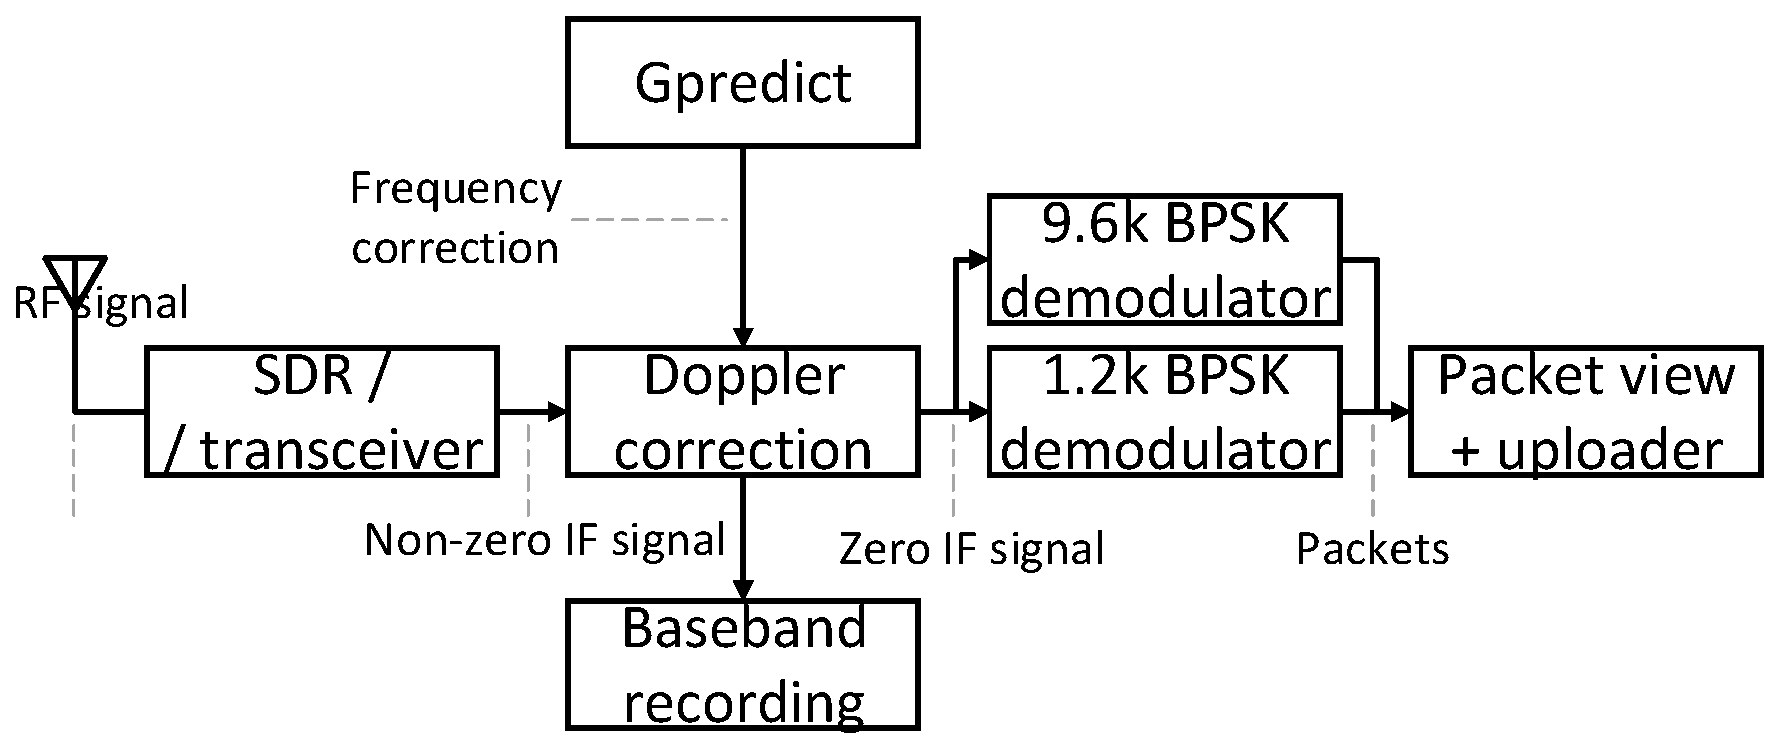
\includegraphics[width=0.6\paperwidth]{img/5/demodulator_block_diagram.eps}
    \caption{Demodulator Block Diagram}
    \label{demodulator_block_diagram}
\end{figure}

First stage, the SDR / transceiver can be any type of Software-Defined radio working with osmocom device drivers, FUNcube SDR or analog SSB radio using audio card. To mitigate the DC-offset and IQ imbalance, the output of this block is on non-zero IF - the frequency of the PW-Sat2 is shifted from the LO frequency. For SSB transceiver, it has to be tuned \SI{2}{\kHz} below the center frequency due to the limited bandwidth of the audio filters. Signal source dialog of the main application is shown in the figure \ref{gs_source_selection}.

\begin{figure}[H]
    \centering
    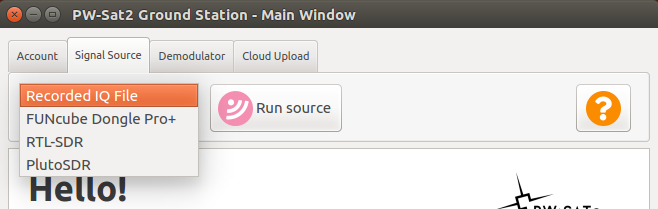
\includegraphics[width=0.6\paperwidth]{img/5/gs_source_selection.png}
    \caption{Ground station application - signal source selection}
    \label{gs_source_selection}
\end{figure}

Doppler correction is build on quadrature mixer and create zero-IF signal for the next processing blocks. Gpredict calculates required frequency shift and sends it to the block via TCP/IP connection. This updates local VCO frequency for the down-conversion. Latter, the signal is fist-stage filtered and saved to the file for logging purposes. GNUradio block diagram is shown in the figure \ref{gs_doppler_gnuradio}.

\begin{figure}[H]
    \centering
    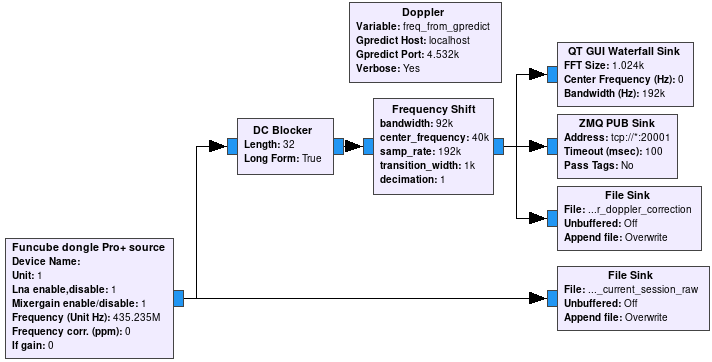
\includegraphics[width=0.6\paperwidth]{img/5/gs_doppler_gnuradio.png}
    \caption{Doppler correction block GNUradio flowgraph}
    \label{gs_doppler_gnuradio}
\end{figure}

In the system, there are two demodulators (for \SI{1.2}{\kbps} and \SI{9.6}{\kbps} bitrates) operating simulateneously. This allows immediate signal reception during bitrate change by the operator without any manual intervention in the software. Each of them consists of couple of blocks, as shown in the figure \ref{gs_demodulator_diagram}. The demodulator has its own GUI  to show user the status of the demodulation, as shown in the figure \ref{gs_demodulator_gui}.
\begin{itemize}
    \item filtering - low-pass signal with matched Root Raised Cosine filter to eliminate out of band noise,
    \item Costas loop - carrier recovery and phase demodulation,
    \item Symbol synchronisation - recovers bits from the baseband signal, locking a PLL onto the signal,
    \item packet framing - builds a frame from stream of bits,
    \item frame pass to the higher level software.
\end{itemize}

\begin{figure}[H]
    \centering
    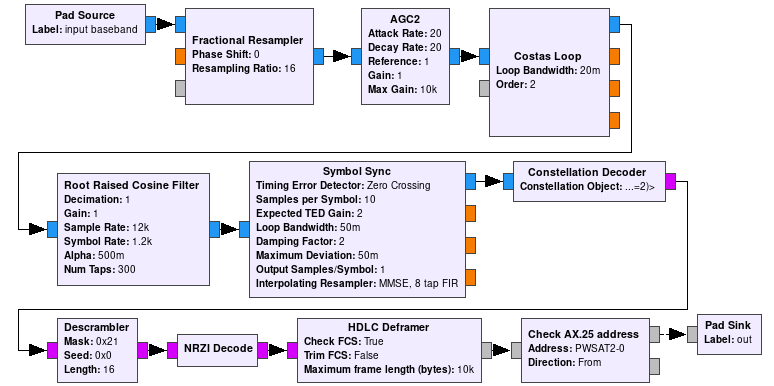
\includegraphics[width=0.6\paperwidth]{img/5/gs_demodulator_diagram.png}
    \caption{Ground station demodulator GNUradio flowgraph}
    \label{gs_demodulator_diagram}
\end{figure}

\begin{figure}[H]
    \centering
    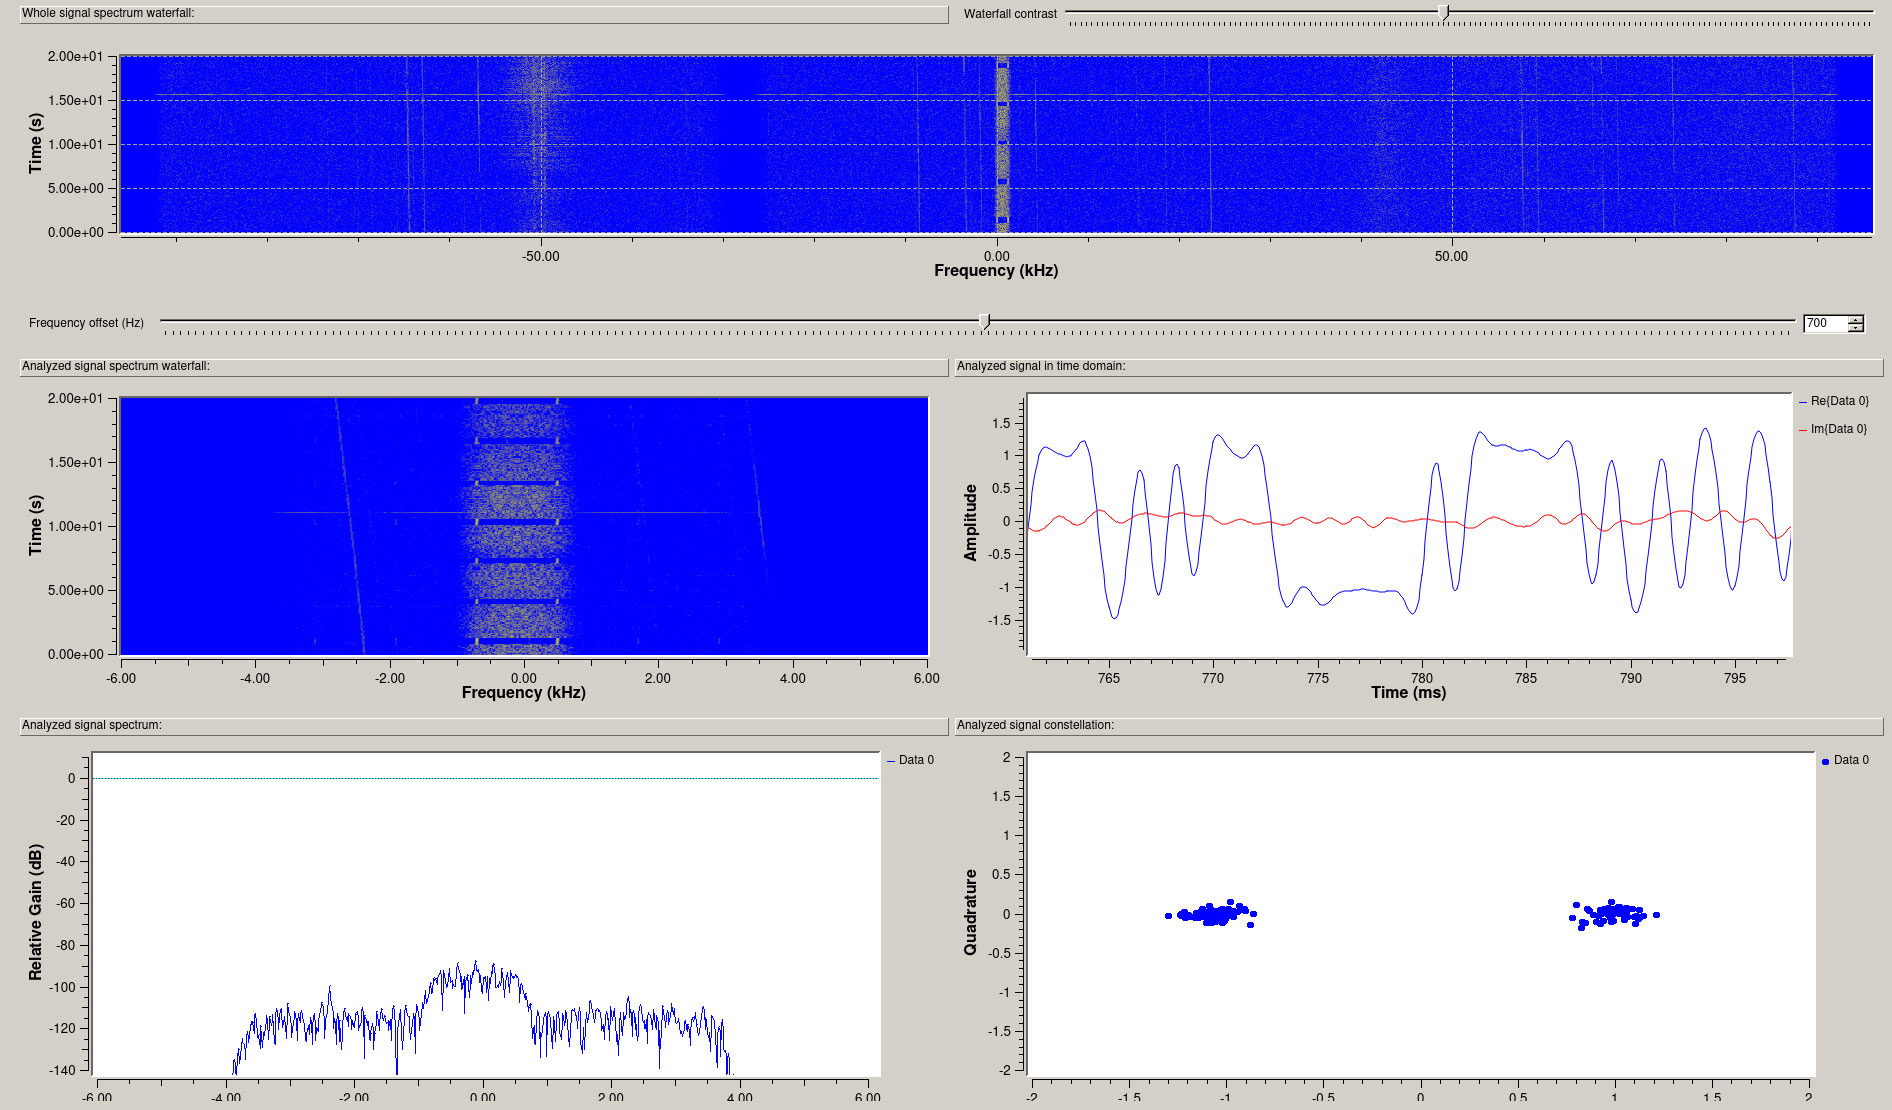
\includegraphics[width=0.6\paperwidth]{img/5/gs_demodulator_gui.jpg}
    \caption{Ground station demodulator GUI}
    \label{gs_demodulator_gui}
\end{figure}

The demodulator was designed for two major cases:
\begin{itemize}
    \item wide bandwidth and large frequency correction (when orbit Keppler data is not well-known, resulting in unpredicted Doppler shift),
    \item wide bandwidth and no frequency correction (when orbit Keppler data is well-known resulting in negligible frequency inaccuracies).
\end{itemize}

Depending on the case, different parameters of the Costa's loop were determined. Both test-cases were implemented and the sensitivity and maximum frequency shift were determined.

After the packet reception, it is shown for the user (as in the figure \ref{gs_frame_view}) and uploaded to the cloud for further analysis by the operations team.

\begin{figure}[H]
    \centering
    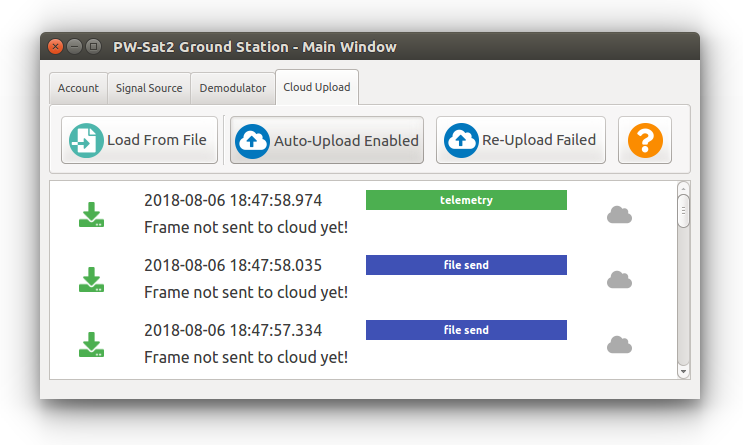
\includegraphics[width=0.6\paperwidth]{img/5/gs_frame_view.png}
    \caption{Ground station received frame view}
    \label{gs_frame_view}
\end{figure}


\subsubsection{Measurements}
Frequency correction block was tested using already flying satellites, verifying stability of frequency after correction.

The test setup for measuring demodulator is shown in the figure \ref{TODO}, and consist of:
\begin{itemize}
    \item PlutoSDR - transmitter of the frames with regulated center frequency and output power,
    \item attenuators
    \item Funcube Pro+ SDR - receiver used in the ground station
\end{itemize}

Frames to be transmitted were recorded with Software-Defined Radio during flatsat campaign and replayed during sensitivity tests. This ensures that all the important inadequacies transmitted by the radio transmitter were also taken into account.
With the test setup, sensitivity was automatically measured by varying output power of the transmitter (in \SI{0.25}{\dB} steps) and PER was recorded for each point. During the process, different parameters of the demodulator were tuned to increase the sensitivity. Final results are shown in the table \ref{TODO} and figures \ref{TODO} - \ref{TODO}.

% \marker[timetimetime-5-ground]

\chapter{Link budget}
The link buget was calculated to estimate the link status, whether the selected component are sufficient to "close" the link. A link budget calculates all of the gains and losses in the radio system, estimating the link margin. In the satellite case, the link budget is a valuable tool - because of the direct line of sight between two communicating nodes, most of the parameters are well known and stable throughout the system lifetime. Main gains from the system comes from: output power of the transmitter and the antennas gain, whereas losses include: free space loss, losses through the medium (atmoshperic losses, ionisation lossed), cable and other in-line devices attenuation, polarisation losses and antenna pointing losses. This section provides an description of the PW-Sat2 link budget, which was based on AMSAT/IARU Link Budget \cite{amsat_link_budget}.

\section{Orbit and slant range}
A slant range (fig \ref{slant_range}) is an maximal distance between the spacecraft and the ground station. It is calculated from the Orbit altitude and the minimal elevation required. For PW-Sat2, useful elevation was assumed at \SI{5}{\degree}. Assumed orbital parameters gives maximum slant range of about \SI{2300}{\kilo\meter} (fig. \ref{slant_range_calc}) and period of \SI{96}{\minute}.

\begin{figure}
    \centering
    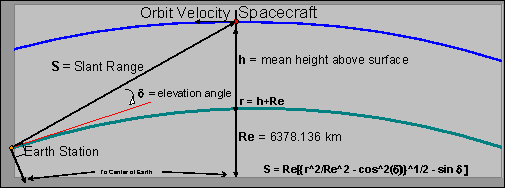
\includegraphics[width=0.8\paperwidth]{img/6/slant_range.pdf}
    \caption{Slant range. Source: \cite{amsat_link_budget}}
    \label{slant_range}
\end{figure}

\begin{figure}
    \centering
    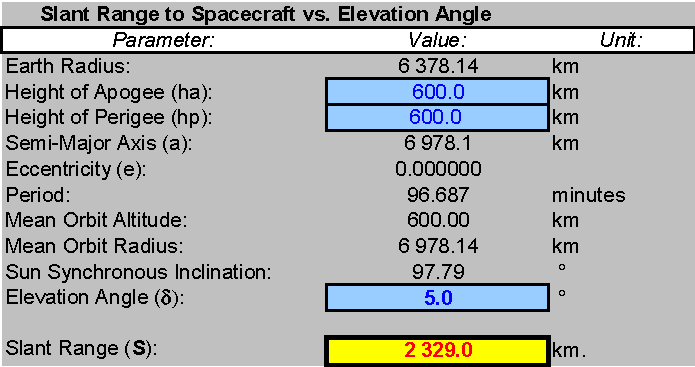
\includegraphics[width=0.8\paperwidth]{img/6/slant_range_calc.pdf}
    \caption{Slant range calculation.}
    \label{slant_range_calc}
\end{figure}

\section{Transmitter capabilities}
The transmitter output power and any in-line losses, as well as antenna mismatch are entered and calculated in the link budget. All the in-line losses are estimated, such as the feeder loss, splitter insertion loss and, if applicable, any other elements, such as the surge protection. The result the power that is actually delivered to the antennas on both the ground station and the spacecraft. The results shown in the figures \ref{link:tx_gs} and \ref{link:tx_spacecraft} indicate the output power \SI{26.63}{\dBm} on the spacecraft and \SI{47.45}{\dBm} on the ground station.

\begin{figure}
    \centering
    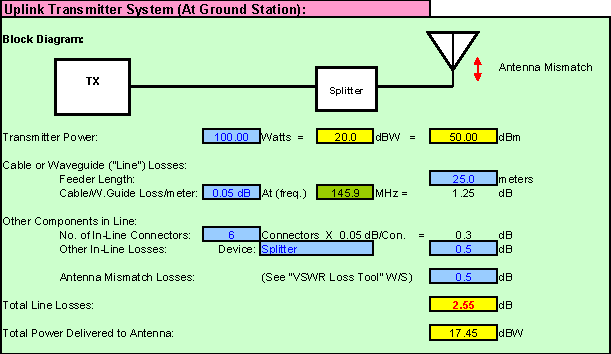
\includegraphics[width=0.8\paperwidth]{img/6/tx_gs.pdf}
    \caption{Ground station output power calculation}
    \label{link:tx_gs}
\end{figure}

\begin{figure}
    \centering
    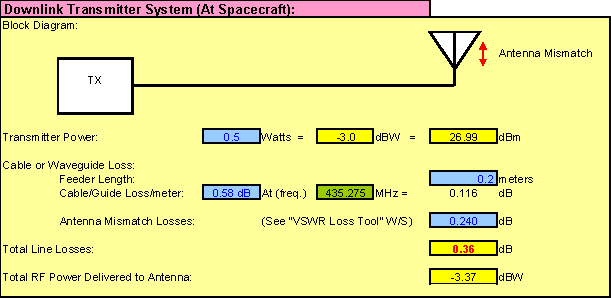
\includegraphics[width=0.8\paperwidth]{img/6/tx_spacecraft.pdf}
    \caption{Spacecraft output power calculation.}
    \label{link:tx_spacecraft}
\end{figure}


\section{Antenna gain}
The antenna gain directly affect the radio link budget. The directional gain of the antennas is taken from the documentation of the manufacturers and for the antennas in the system they are equal to:
\begin{itemize}
    \item Ground station - Cross-Yagi antennas, \SI{13.2}{\dBi} for uplink, \SI{16.2}{\dBi} for downlink,
    \item Spacecraft - both antennas are dipoles, \SI{2.15}{\dBi} as for ideal dipole is assumed as the antennas are working in the resonance. 
\end{itemize}


\section{Medium losses}
The main signal loss in the spacecraft communication comes from the Free space loss, given by the formula: $\text{Loss [dB]} = 22 + 20 \cdot \log_{10} (\text{d}/\lambda)$, where $d$ - distance in meters, $\lambda$ - wavelength. Other sources of losses taken into the consideration for the sub-GHz bands are atmospheric losses and losses in the ionosphere. Atmospheric absorption strongly depends on the total number of molecules along the path between the spacecraft and the ground station - therefore the elevation angle. Losses due to the atmospheric gases are nearly independent of atmospheric temperature, density and relative humidity at frequencies below 2 GHz. \cite{sat_propagation}. At \SI{5}{\degree} elevation, the atmospheric are estimated at \SI{2.1}{\dB}. The ionosphere limits the lowest frequency at which satellite communications is possible. Below \SI{20}{\MHz}, during solar maximum, signals are usually fully absorbed or reflected by the layers of the ionosphere. VHF, UHF and Microwave frequencies are influenced far less amount, but the value of the attenuation varies with time. For the purpose of calculation above \SI{100}{\MHz} is is sufficient to estimate losses in the ionosphere as below \SI{1}{\dB}.

Total medium losses are equal:
\begin{itemize}
    \item Uplink - \SI{145.9}{\MHz} - $FSPL = \SI{146.2}{\dB}$
    \item Downlink - \SI{145.9}{\MHz} - $FSPL = \SI{155.7}{\dB}$
\end{itemize}


\section{Polarization losses}
On the ground station, both antennas has circular polarization, whereas on the spacecraft, antennas are linearly polarized. This eliminates the effect of signal strength variance with the rotation of the satellite, but only the half power is received by the antennas. The polarization loss of \SI{3}{\dB} was assumed in both uplink and downlink.

\section{Antenna pointing losses}
Antenna pointing losses are exhibited when the maximal directivity gain of the antennas are not aligned with the receiver (fig. \ref{link:pointing_loss}). For ground station, the rotator and its controller are pointing with the accuracy of about \SI{1}{\degree} but due to the wind and other non-ideal factors the pointing error was assumed for \SI{5}{\degree}. The antenna gain loss was read from the radiation patterns (fig. \ref{radiation_144} and \ref{radiation_435}) as estimated at \SI{1}{\dB}. For the spacecraft, as the antennas have dipole characteristics, they are mostly omnidirectional, but with significant drops in the directivity along the dipole axis. The communication will break at some angles along the dipole axis, is was assumed that the coverage of \si{300} per \SI{360}{\degree} is sufficient. At standard dipole roll-off factor (fig. \ref{link:dipole_pattern}), \SI{70}{\degree} pointing error equals to \SI{4.7}{\dB} pointing loss.

\begin{figure}
    \centering
    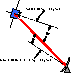
\includegraphics[width=0.5\paperwidth]{img/6/pointing_loss.pdf}
    \caption{Pointing losses. Source: \cite{amsat_link_budget}}
    \label{link:pointing_loss}
\end{figure}

\begin{figure}
    \centering
    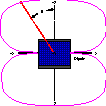
\includegraphics[width=0.4\paperwidth]{img/6/dipole_pattern.pdf}
    \caption{Dipole antenna radiation pattern. Source: \cite{amsat_link_budget}}
    \label{link:dipole_pattern}
\end{figure}


\section{Antenna temperature}
For receiver antennas the antenna temperature is the total noise figure added by the antenna which come from other sources than transmitter of interest. It adds to the noise produced by the Low Noise Amplifier, resuling in lowering the Signal To Noise ratio.
The sky temperature as seen by a spacecraft must be viewed from its perspective. In the beamwidth of the omnidirectional antenna on Low Earth Orbit there is a half of a sphere of the deep space and half of the Earth. The sky itself which is nominally at \SI{2.7}{\kelvin} but, at frequencies below \SI{2}{\GHz} also includes galactic noise, which is highest in directions that intercept the disk of the Milky Way.  At \SI{146}{\MHz} this value can be as high as \SI{1700}{\kelvin} and as low as \SI{80}{\kelvin} \cite{amsat_link_budget}. The average Earth temperature used is \SI{290}{\kelvin}, however, the Earth may be warmer due to man-made noise sources that can be distributed on the surface of the planet. The average antenna temperature of the spacecraft was assumed to $0.5 \cdot \SI{70}{\kelvin} + 0.5 \cdot \SI{330}{\kelvin} = \SI{200}{\kelvin}$.
For a ground station antenna the Sky Temperature value must include not only the noise intercepted by the ground station antenna coming from the colder sky into which the antenna is looking but, it has to include any terrestrially generated noise that may be generated in the proximity of the station. This condition is worst when the ground station antenna is at low elevation angles and pointed in the direction of the source of the noise. For PW-Sat2, the receiver antenna is placed in the middle of the Warsaw, resulting in increased temperature depending on the azimuth of the antenna. During ground station calibration, the power spectrum density was measured using spectrum analyzer, resulting in the noise floor of about \SI{-132}{\dBm} in \SI{10}{\kHz} RBW. This implies the antenna temperature of about \SI{500}{\kelvin}.


\section{Receiver performance}
The receiver performance was measured for both uplink and downlink using the attenuators and packet transmitters. During the sensitivity tests, the "effective" antenna temperature was \SI{290}{\kelvin} - the noise was produced by the electrical components in the room temperature. This means that during the mission, the sensitivity will be affected by the noise added by the antenna.
For uplink, the effective sky antenna (\SI{200}{\kelvin}) is actually lower then the room temperature, meaning that the sensitivity of the system will improve by $10\cdot \log_{10}(200/290) = \SI{1.6}{\dB}$, resulting in receiver sensitivity for \SI{1}{\percent} PER: \SI{-98}{\dBm}.
In the ground station the effective antenna temperature will be higher than during tests on the bench, resulting in the reduce of the sensitivity by $\SI{2.3}{\dB}$. This gives the effective sensitivity at \SI{-124}{\dBm}.


\section{Link budget summary}
Summing all the gains and losses produces a valuable overview of the system performance (fig. \ref{link:link_status}). The power on the receiver ports of the system are calculated and compared to the sensitivities of the receivers, resulting in link status and margin. The link margins are above \SI{5}{\dB} - the safe limit and are equal to \SI{6.0}{\dB} for downlink and \SI{5.7}{\dB} for uplink. Most of the time the performance will be better due to the lower pointing losses of the spacecraft. 

\begin{figure}
    \centering
    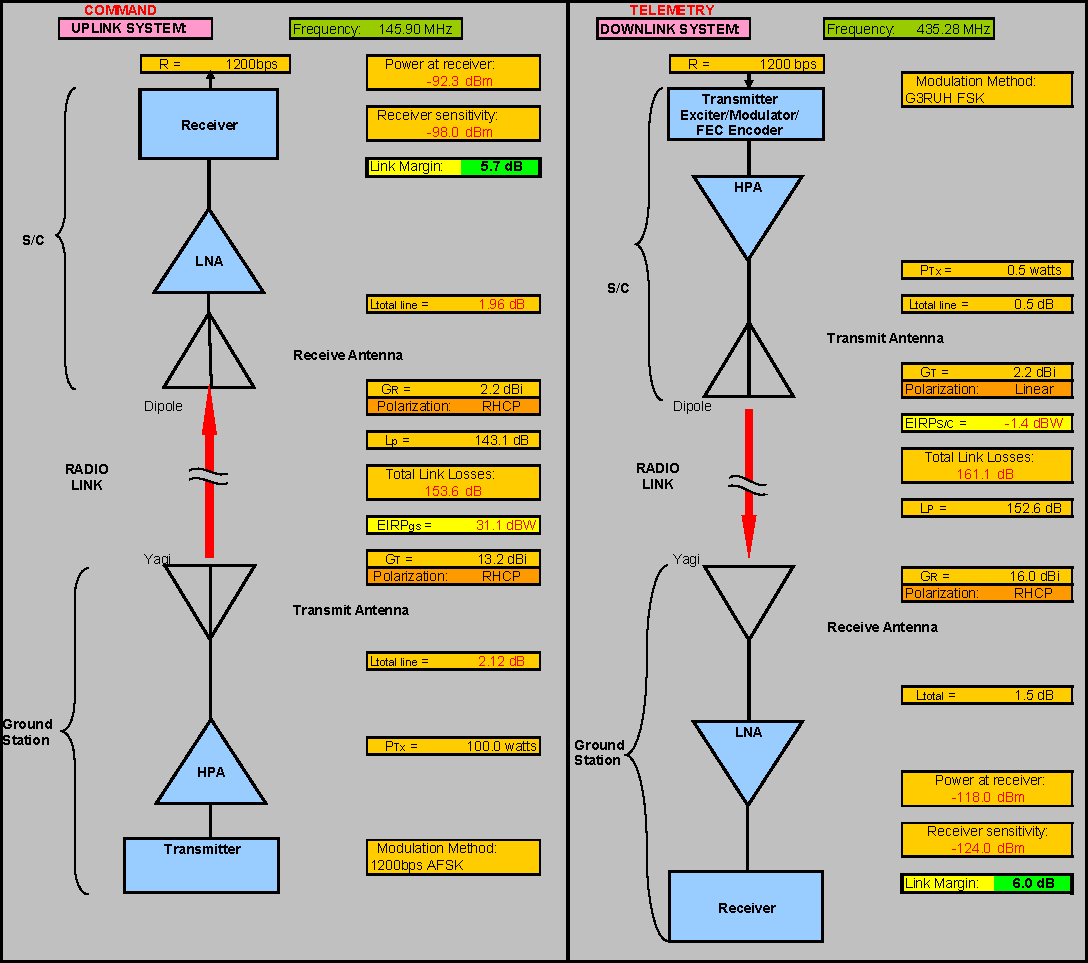
\includegraphics[width=0.8\paperwidth]{img/6/link_summary.pdf}
    \caption{System performance summary.}
    \label{link:link_status}
\end{figure}
% % \marker[timetimetime-6-results]

\chapter{Mission results}
At $3^{rd}$ of December 2018, PW-Sat2 was launched on \SI{590}{\kilo\meter} orbit on-board Falcon9 rocket from SpaceX company. 

\section{Lanuch and Early Operations Phase}
During first hours after launch, PW-Sat2 was inside the container, completely turned off by the hardware kill-switch. 4 hours after the launch, it was deployed and turned on automatically. On-Board software, after silent period of \SI{30}{\minute} performed antenna deployment procedure and started transmitting beacon data every \SI{60}{\second}.

%TODO http://k4kdr.github.io/
Beacon data (consisting of satellite telemetry) was received first by Scott Chapman (K4KDR) from United States of America at 6:10 am the day after launch. Later, during the first couple of days of orbital operations the Bus and Payload commissionings were performed.

During first sessions, satellite was transmitting with \SI{1200}{\bps} downlink speed, providing reliable radio link. PW-Sat2 took first polish satellite photograph TODO at $5^{th}$ of December 2018. It was taken by a part of camera built-in tests and downloaded on request from ground.


\section{Doppler correction}
During the launch, \si{64} satellites were launched together and were separated from the upper stage of the rocket by spring actions. At first, they were flying together and with the time, they were further apart from each other. Figure TODO show the on-orbit position of the satellites on \si{25^{th}} day after the launch. Doppler effect estimation was performed during every pass, with increased accuracy. Typical method for selecting an satellite object from a set of different ones is done by applying Doppler correction to the received signal spectrum, for every object in the field of view, and later choosing the most suited one. 

Signal before and after Doppler correction is shown in the figure \ref{Doppler_correction_gqrx}.

\begin{figure}
    \centering
    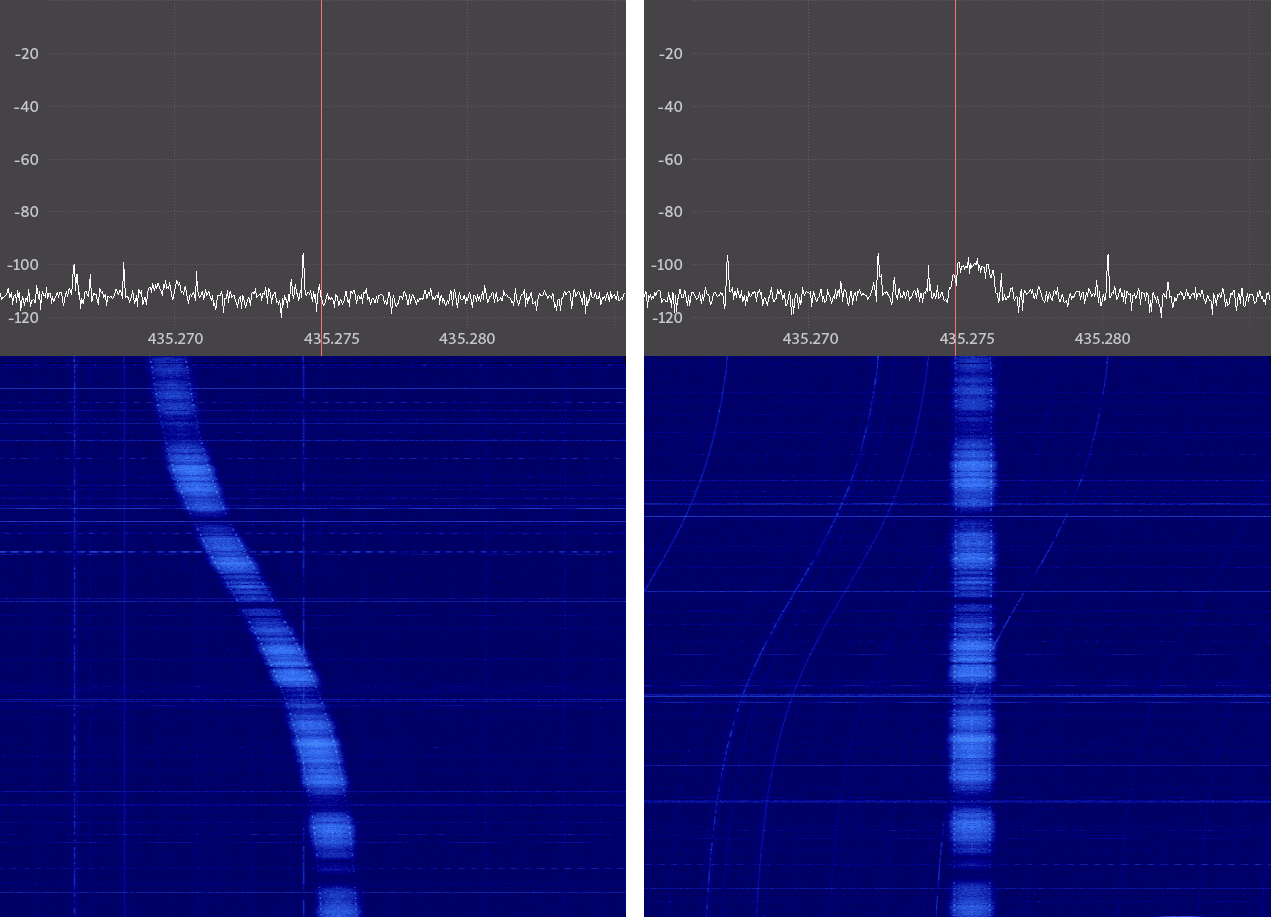
\includegraphics[width=0.65\paperwidth]{img/7/doppler_correction.png}
    \caption{Doppler correction.}
    \label{Doppler_correction_gqrx}
\end{figure}

\section{Link budget estimation}


\section{Main mission results}



% \marker[timetimetime-6-results]

\appendix
\printbibliography

\marker[timetimetime-7-end]

\end{document}
